\documentclass[a4paper, 11pt]{report}
\usepackage[a4paper, margin=2.5cm]{geometry}

% Police
\usepackage{libertine}

% Interlignes et paragraphes
\usepackage{setspace} % pour l'interligne
\usepackage{parskip}  % pour gérer l'espacement entre les paragraphes

% Interligne multiple de 1.15
\setstretch{1.15}

% Espace après paragraphe : 6pt
\setlength{\parskip}{6pt}
\setlength{\parindent}{15pt} % Retrait en début de paragraphe

\usepackage{lmodern}
\usepackage[french]{babel}
\usepackage[utf8]{inputenc}
\usepackage[T1]{fontenc}

\usepackage{graphicx} % Pour les images
\graphicspath{Figures}
\usepackage{caption}
\usepackage{siunitx} % for S column in tabular
\usepackage{subcaption}
\usepackage{amsmath, amsfonts, amssymb} %Pour les maths

\usepackage{textcase}

\usepackage{afterpage}

% La numérotation

\makeatletter\@addtoreset{section}{chapter}\makeatother
\renewcommand{\thepart}{\Roman{part}}
\renewcommand{\thechapter}{\arabic{chapter}}
\renewcommand{\thesection}{\Roman{section}}

\usepackage{chngcntr}
\counterwithin{figure}{section}

% Sommaire + hyperliens

\usepackage[hyphens]{url}
\usepackage[pdfauthor = {{Julien Sagnes}}, pdftitle = {{Rapport de Projet}}, pdfstartview = Fit, pdfpagelayout = SinglePage, pdfnewwindow = true, bookmarksnumbered = true, breaklinks, colorlinks, linkcolor = black, urlcolor = black, citecolor = black, linktoc = all]{hyperref}
\usepackage[
    left = \flqq{},% 
    right = \frqq{},% 
    leftsub = \flq{},% 
    rightsub = \frq{} %
]{dirtytalk} % permet de citer mieux

% Codes

\usepackage{booktabs}
\usepackage{listings}
\usepackage{xcolor}
\usepackage[section]{placeins}
\usepackage{enumitem}
\usepackage{accsupp}

\newcommand{\noncopynumber}[1]{%
    \BeginAccSupp{method=escape,ActualText={}}%
    #1%
    \EndAccSupp{}%
}

\definecolor{codegreen}{rgb}{0,0.6,0}
\definecolor{codegray}{rgb}{0.5,0.5,0.5}
\definecolor{codepurple}{rgb}{0.58,0,0.82}
\definecolor{backcolour}{rgb}{0.95,0.95,0.92}

\lstdefinestyle{mystyle}{
    backgroundcolor=\color{backcolour},   
    commentstyle=\color{codegreen},
    keywordstyle=\color{magenta},
    numberstyle=\tiny\color{codegray},
    stringstyle=\color{codepurple},
    basicstyle=\ttfamily\footnotesize,
    breakatwhitespace=false,         
    breaklines=true,                 
    captionpos=b,                    
    keepspaces=true,                 
    numbers = left,
    numberstyle=\tiny\noncopynumber,
    numbersep=5pt,                  
    showspaces=false,                
    showstringspaces=false,
    showtabs=false,                  
    tabsize=2,
    literate=
  {á}{{\'a}}1 {é}{{\'e}}1 {í}{{\'i}}1 {ó}{{\'o}}1 {ú}{{\'u}}1
  {Á}{{\'A}}1 {É}{{\'E}}1 {Í}{{\'I}}1 {Ó}{{\'O}}1 {Ú}{{\'U}}1
  {à}{{\`a}}1 {è}{{\`e}}1 {ì}{{\`i}}1 {ò}{{\`o}}1 {ù}{{\`u}}1
  {À}{{\`A}}1 {È}{{\'E}}1 {Ì}{{\`I}}1 {Ò}{{\`O}}1 {Ù}{{\`U}}1
  {ä}{{\"a}}1 {ë}{{\"e}}1 {ï}{{\"i}}1 {ö}{{\"o}}1 {ü}{{\"u}}1
  {Ä}{{\"A}}1 {Ë}{{\"E}}1 {Ï}{{\"I}}1 {Ö}{{\"O}}1 {Ü}{{\"U}}1
  {â}{{\^a}}1 {ê}{{\^e}}1 {î}{{\^i}}1 {ô}{{\^o}}1 {û}{{\^u}}1
  {Â}{{\^A}}1 {Ê}{{\^E}}1 {Î}{{\^I}}1 {Ô}{{\^O}}1 {Û}{{\^U}}1
  {œ}{{\oe}}1 {Œ}{{\OE}}1 {æ}{{\ae}}1 {Æ}{{\AE}}1 {ß}{{\ss}}1
  {ű}{{\H{u}}}1 {Ű}{{\H{U}}}1 {ő}{{\H{o}}}1 {Ő}{{\H{O}}}1
  {ç}{{\c c}}1 {Ç}{{\c C}}1 {ø}{{\o}}1 {å}{{\r a}}1 {Å}{{\r A}}1
  {€}{{\EUR}}1 {£}{{\pounds}}1
}
\lstset{style=mystyle}

\begin{document}

\definecolor{darkWhite}{rgb}{0.94,0.94,0.94}

% Page de garde

\begin{titlepage}
    \newcommand{\HRule}{\rule{\linewidth}{0.5mm}}
    \begin{center}
        \begin{minipage}{1\linewidth}
            \begin{flushleft}
                \hspace{4.5cm}
                
\includegraphics[width=0.25\textwidth]{Figures/SORBONNE_FAC_SCIENCES_DEF_CMJN.pdf}
            \end{flushleft}
        \end{minipage}

        \vspace{1.5cm}
        
        \textsc{\Large{}Master SAR 1\up{\MakeTextLowercase{ère}} année} \\[0.5cm]
        \textsc{\large{}2024 - 2025} \\[0.5cm]

        \HRule \\[0.6cm]
        {\huge\bfseries{}Rapport de projet :} \\
        \LARGE{Conception et dimensionnement d'une pince robotique à trois doigts flexibles} \\[0.25cm]
        \HRule \\[1.5cm]


        \Large\textit{Auteurs :}\\
        \begin{center}
            Julien \textsc{Sagnes}\\
            Minh \textsc{Nhut Nguyen}
        \end{center}

        \hfill

        \Large\textit{Responsable :}\\
        \begin{center}
            Faiz \textsc{Ben Amar}
        \end{center}
        \vspace{1cm}
        {\large\today} \\[2cm]
    \end{center}

    \vfill
\end{titlepage}


\selectlanguage{french}
% Résumé sur une page séparée avant la table des matières
\clearpage
\section*{Résumé}
\addcontentsline{toc}{section}{Résumé}
Ce document présente la conception et le dimensionnement d'une pince robotique à trois doigts flexibles. Blablabla...

\clearpage
\tableofcontents
\clearpage

\section{Introduction}

    Dans l'industrie, la robotique collaborative, ou cobotique, est omniprésente. Elle vise à soulager l’être humain en prenant en charge les tâches pénibles, notamment à l’aide de préhenseurs conçus spécifiquement pour manipuler des charges de tailles et de poids variables, souvent associées à des tâches répétitives. \cite{noauthor_cobotique_nodate}

    Ce projet consiste à concevoir et dimensionner une pince robotique à trois doigts flexibles, conçue pour s'ouvrir et se refermer en s'adaptant à l'objet saisi. L'objectif est de réussir à attraper des fruits et légumes relativement légers, comme un poivron. Nous utiliserons \textit{SolidWorks} pour modéliser le robot, et étudierons son élasticité par éléments finis via \textit{SolidWorks Simulation}.

    Elle sera ensuite fixé au bras robotique...

    \subsection{Motivations et principes fondamentaux}

        \begin{figure}
            \centering
            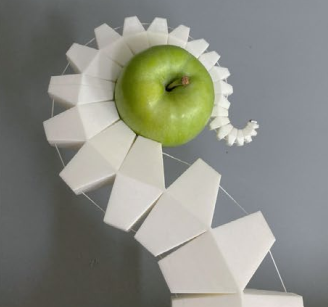
\includegraphics[width=0.5\textwidth]{Figures/pieuvre.png}
            \caption{Inspiration du SpiRob pour les 3 doigts de notre pince \cite{wang_spirobs_2025}}
            \label{fig:pieuvre}
        \end{figure}
    
        Dans notre cas, et comme souvent en robotique, les objets à manipuler ont une forme ou une position mal connue, et contrairement à une main humaine, les pinces robotiques manquent de retour tactile fiable. Pour cette raison, nous n'allons pas utiliser de retour haptique, mais plutôt de préhenseurs souples. Nous nous inspirons de la flexibilité des tentacules de pieuvre (voir figure \ref{fig:pieuvre}), ce qui permettra à la pince de s'adapter naturellement à la forme de divers fruits et légumes, sans nécessiter de capteurs ni de système de contrôle complexe, simplement grâce à la compliance mécanique.
        
        La compliance désigne la capacité d’un robot à adapter la rigidité de ses mouvements en fonction des forces extérieures. Autrement dit, il ajuste naturellement sa posture pour bien épouser l’objet qu’il manipule. Dans ce projet, nous nous concentrons sur la compliance passive, où la structure mécanique du robot est suffisamment flexible pour se déformer sous l'effet d'une contrainte externe. Cette approche permet une préhension polyvalente et adaptable. \cite{noauthor_gestion_2016}

        Malgré ses avantages, cette flexibilité favorise le flambage sous de grandes forces d'actionnement et limite donc la charge maximale. Il faut donc établir un compromis sur la souplesse, afin d'assurer la flexibilité et la capacité à soutenir des charges raisonnables. \cite{wang_spirobs_2025}
    
    \subsection{Comportement et structure de la pince}
    
        La pince pourra adopter deux configurations distinctes : ouverte ou fermée. Elle sera haute de 10 cm en position ouverte et composée de 3 doigts identiques soumis à un encastrement rigide sur une base. Les doigts seront positionnés symétriquement autour du centre de la base, chacun séparé par un angle de 120°. Des câbles passeront de chaque côté des doigts et permettront de les contrôler. L'actionnement à câbles peut être localisé sur la la base ou déporté à l'extérieur du système, il sera question d'effectuer une étude comparative des différentes solutions possibles.
        
        La flexion de chaque doigt sera assurée par une force appliquée sur le câble situé du côté fléchisseur par l'utilisation d'un moteur, tandis que le retour à la position initiale se fera naturellement, cette dernière devant être la position d'équilibre lorsque le moteur n'exerce plus de couple. Il est donc crucial de dimensionner correctement les doigts et les câbles afin qu'ils conservent un comportement élastique et réversible, sans déformation permanente. C'est pourquoi nous utiliserons un matériau souple qui puisse se plier sans se casser, le TPU, en prenant soin de ne pas aller dans le domaine plastique. Par la suite, nous étudierons les flexions, les contraintes maximales et le retour élastique afin de s'assurer de ne pas rentrer dans le modèle plastique.
                
        Enfin, il sera essentiel de garantir autant que possible la répétabilité, un aspect souvent problématique dans le domaine de la robotique flexible, car la souplesse peut introduire des incertitudes sur la position exacte des doigts.

    \subsection{Choix de l'actionneur et des câbles}

        Nous devons choisir entre un moteur rotatif actionnant un tambour et un moteur linéaire. Si nous optons pour un moteur rotatif avec un tambour, il est crucial d'éviter que le câble ne s'enroule sur lui-même. Étant donné que la course du câble est calculée en fonction de la rotation du moteur, il est essentiel que le câble ne tourne pas sur lui-même pour éviter de fausser les résultats. Nous pourrions envisager une glissière pour guider l'enroulement du fil le long d'un axe, ou un mécanisme utilisant une vis sans fin pour maintenir la tension.

        Dans les systèmes mécaniques utilisant des câbles ou des tendons, la tension est essentielle pour assurer une transmission efficace de la force ou du mouvement. Une tension insuffisante peut entraîner un glissement, un flambage et une perte de performance. Idéalement, la tension dans le câble doit être directement liée à la force produite par le moteur. Ainsi, la force appliquée par le moteur doit être transmise directement et efficacement au câble sans perte significative. C'est pourquoi nous étudierons l'idée d'utiliser des réducteurs d'engrenage avec un rapport de réduction de 6 à 10 pour éviter les pertes, de sorte que la tension dans le câble reflète celle du moteur.

        Il est également question de choisir des fils optimaux pour la conception du robot. Si nous utilisons des fils de pêche, nous devons résoudre le problème de la souplesse du fil qui peut flamber lorsque le robot revient à sa position d'équilibre. Une solution pourrait être d'accompagner le mouvement avec le moteur pour limiter sa vitesse et contrôler en permanence la tension du câble. Nous pourrions également utiliser des câbles en acier pour éviter ce phénomène de flambage, mais dans ce cas, la solution du tambour serait inopérante.
        
\clearpage

\section{État de l'art}

    \subsection{Préhenseurs souples}

        Dans un premier temps nous voyons rapidement l'intérêt des préhenseurs souple à travers deux exemples.

        \subsubsection{Étude d'une pince en PVC}
            
            \begin{figure}[htbp]
                    \centering
                    \begin{subfigure}[t]{0.8\textwidth}
                        \centering
                        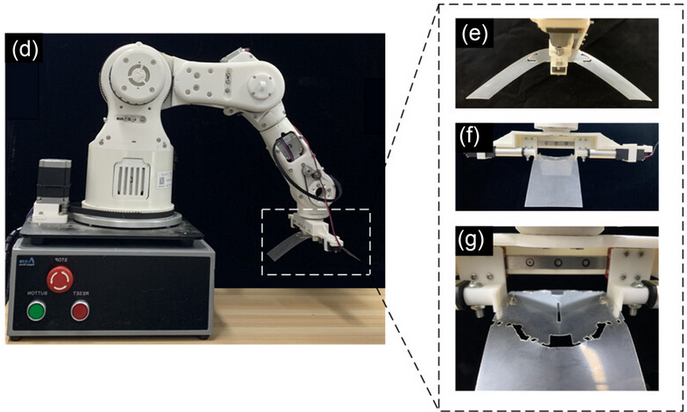
\includegraphics[width=\textwidth]{Figures/robot.png}
                        \caption{Robot Anno V6-PLUS qui porte la pince \cite{liu_origami_2023}}
                    \end{subfigure}
                    \hfill
                    \begin{subfigure}[t]{0.8\textwidth}
                        \centering
                        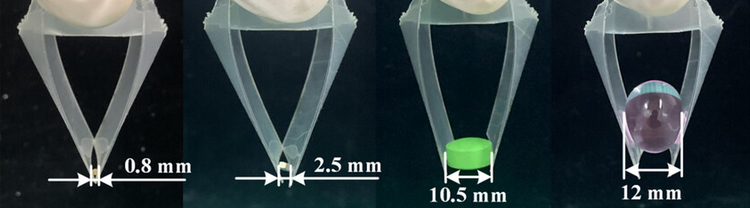
\includegraphics[width=\textwidth]{Figures/adaptability.png}
                        \caption{Exemples d'utilisation de la pince souple \cite{liu_origami_2023}}
                    \end{subfigure}
                    \caption{Illustration de l'étude sur la pince souple}
                    \label{fig:origami}
                \end{figure}
        
            Une étude a été menée afin de concevoir des préhenseurs souples en origami, permettant une adaptabilité de préhension pour de nombreux objets. La pince, qui n'est qu'une simple feuille de PVC (voir figure \ref{fig:origami}.a.(e)), est commandée grâce à un moteur linéaire. Le moteur linéaire est fixé au bras robotique via un support (bracket). Ce moteur est relié à un poussoir qui coulisse sur une glissière. Lorsqu’on alimente le moteur linéaire, il pousse ou tire le poussoir de manière rectiligne. Le mouvement du poussoir est ainsi transmis à la pince flexible, qui s’ouvre ou se ferme selon la direction du mouvement. Afin de garantir la stabilité, un cadre de limitation empêche le poussoir de dépasser certaines positions, et le système de guidage symétrique (les deux extrémités du poussoir étant à la même hauteur) empêche la pince de se déformer de manière asymétrique, ce qui garantit une prise stable (voir figure \ref{fig:origami}.a.(g)). \cite{liu_origami_2023}.
    
            Cette étude démontre que même une structure souple minimaliste peut offrir une adaptation efficace à des objets de formes variées. En effet, comme nous pouvons le remarquer sur la figure \ref{fig:origami}.b, la pince souple s'adapte parfaitement à chaque taille d'objet pour le même effort à son extrémité.

        \subsubsection{Étude d'une pince flexible multi-stable à l'aide du kirigami}
    
            \begin{figure}
                \centering
                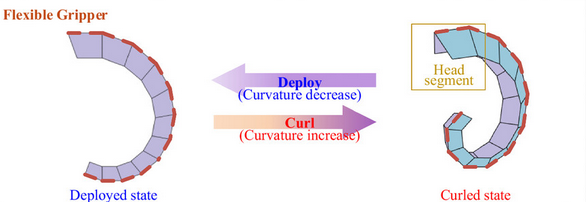
\includegraphics[width=0.7\textwidth]{Figures/multi-stable.png}
                \caption{Pince à plusieurs positions stables \cite{qi_kirigami_2024}}
                \label{fig:multi_stable}
            \end{figure}
    
            Cette étude \cite{qi_kirigami_2024} explore la conception d'une pince souple en s'appuyant sur les principes du kirigami, une technique dérivée de l'origami. Cette approche permet de générer des structures à multi-stabilité passive, c’est-à-dire capables de maintenir plusieurs configurations d’équilibre, notamment une configuration pince fermée et une autre pince ouverte (voir figure \ref{fig:multi_stable}). Ce changement de configuration s'opère grâce à une structure "trigger" (déclencheuse) capable de convertir une force longitudinale appliquée en un mouvement de déformation latérale des bras de la pince.
    
            Néanmoins, l’approche présente aussi des limites, notamment en termes de force de préhension. La pince kirigami décrite utilise des actionneurs diélectriques ou des forces manuelles pour effectuer la transition de forme, ce qui restreint sa capacité à soulever des charges importantes. Cela la rend peu adaptée aux applications où une capacité de charge élevée est requise — comme c’est le cas dans notre projet où l’objectif est de manipuler des objets jusqu’à 5 kg. Enfin, bien que le système ne repose pas sur une action par câble comme notre pince inspirée du SpiRob, cette étude permet de souligner que les principes de déformation géométrique contrôlée et de multi-stabilité passive constituent une piste intéressante pour notre pince.
    
    \subsection{Actionnement par câbles}

        Deuxièmement, nous établissons une synthèse utile sur l'actionnement par câbles.
    
        \subsubsection{Étude de la spirale logarithmique avec le SpiRob}
        
            \begin{figure}
                \centering
                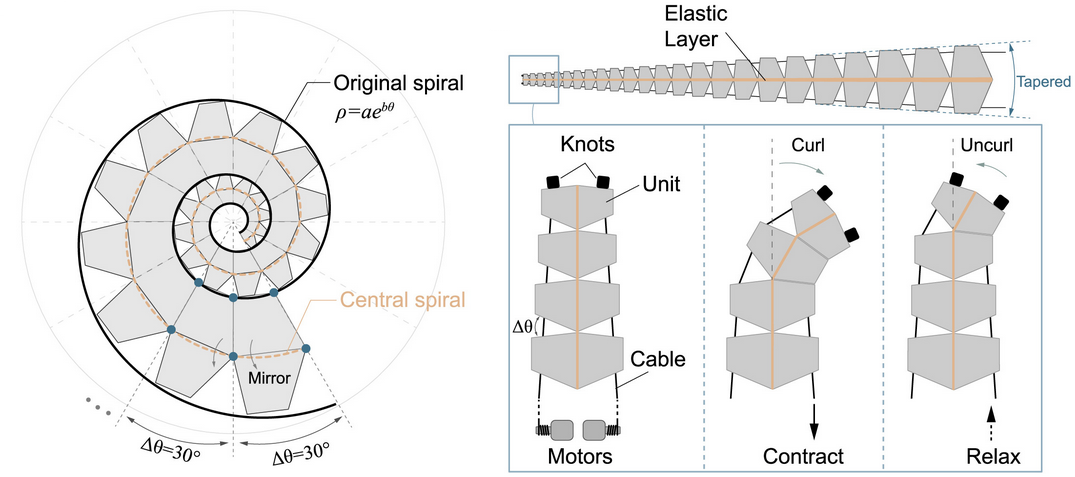
\includegraphics[width=1.0\textwidth]{Figures/spiral_logarithm.png}
                \caption{Spiral logarithmique du préhenseur \cite{wang_spirobs_2025}}
                \label{fig:spiral_logarithm}
            \end{figure}
    
            Les câbles sont utilisés pour activer le mouvement de curling (enroulement) et uncurling (déroulement) des SpiRobs, des robots souples en forme de spirale logarithmique inspirés des appendices biologiques (bras d'octopus, trompe d'éléphant).

            Un ou plusieurs câbles (2 pour les robots 2D, 3 pour les robots 3D) passent à travers des trous percés dans les unités du robot. Une extrémité est fixée à l'unité la plus distale (pointe du robot) par un nœud de pêcheur, et l'autre est connectée à un moteur (voir figure \ref{fig:spiral_logarithm}). La contraction des câbles enroule le robot en une spirale logarithmique, tandis que leur relâchement le ramène à sa position d'équilibre grâce à son élasticité. En effet, le TPU que constitue le robot permet ce comportement. 

            Les auteurs ajoutent également un amortissement pour limiter la vitesse du mouvement et assurer le contrôle de la tension des câbles. Une règle linéaire ($F_1^0 = -c_1 p + c_2 \alpha + c_0$) ajuste la force antagoniste au mouvement en fonction de la position de l'objet ($p, \alpha$) en coordonnées polaires par rapport à la position de l'extrémité du robot, avec des coefficients expérimentaux ($c_0=14, c_1=13, c_2=5$). Cela permet une saisie automatique avec un taux de succès de 94,4 $\%$. En somme, Plus l'objet est éloigné, plus la force antagoniste à laquelle le robot est soumis est faible. \cite{wang_spirobs_2025}

            Du reste, les SpiRobs sont entièrement réalisés en \textbf{TPU (Thermoplastic Polyurethane)}, un matériau souple imprimé en 3D à l’aide de filaments eTPU-95A (shore A95). Ce choix permet une bonne compliance mécanique tout en maintenant une certaine rigidité, indispensable pour transmettre efficacement la tension appliquée par les câbles. Le TPU confère aux robots une capacité à s’enrouler en spirale logarithmique puis à se redéployer, sans nécessiter d’articulations ni de moteurs multiples. Le retour à l’état initial est assuré par une couche centrale élastique jouant le rôle de ressort passif. \cite{wang_spirobs_2025}

            Par ailleurs, l'angle de conicité de la spirale joue un rôle clé dans les performances de préhension du doigt, notamment en termes d’espace de travail, de précision de saisie et de capacité de charge. 
            D’après les résultats rapportés dans \cite{wang_spirobs_2025}, un \textbf{faible angle de conicité} permet d’augmenter significativement l’espace de travail, en élargissant la zone accessible par les doigts lors du déploiement. À l’inverse, un \textbf{angle de conicité plus élevé} améliore la performance de saisie : il permet de saisir des objets de plus petite taille (diamètre minimal réduit) tout en augmentant la \textbf{capacité de charge maximale} du robot.
            À géométrie constante, l’augmentation du poids de l’objet à saisir est également mieux tolérée lorsque le diamètre est grand, ce phénomène étant particulièrement marqué pour les objets volumineux. Par exemple, un SpiRob avec un angle de conicité de $15^\circ$ peut saisir des objets dont le diamètre varie de \textbf{5{,}6\,mm à 115\,mm}, et supporter une charge allant jusqu’à \textbf{10\,kg}, soit environ \textbf{260 fois son propre poids} (poids du robot : 38{,}4\,g). \cite{wang_spirobs_2025}

            On observe alors plusieurs problèmes rencontrés auxquels il faudra penser lors de la conception. Il s'agit de limiter les frottements entre les câbles et le corps du robot (une friction élevée peut causer des pertes d'énergie, des déformations non uniformes, ou un phénomène de flambage des fils), mais il faut aussi éviter d'avoir une couche élastique trop épaisse (au centre du robot), car cela augmenterait la force nécessaire pour enrouler le robot, rendant l'actionnement par câbles plus exigeant pour les moteurs qui utiliseraient alors davantage d'énergie. Pour régler la friction des câbles, nous pouvons utiliser des câbles UHMWPE pour leur faible coefficient de frottement et leur résistance à l'usure. Quant à l'optimisation de la couche élastique, une épaisseur de couche élastique de 5 $\%$ est optimale d'après les tests effectués, assurant une bonne élasticité sans nécessiter une force excessive pour l'enroulement \cite{wang_spirobs_2025}.

        \subsubsection{Étude des systèmes de transmissions et d'actionnements par câble pour des exosuits}

            \begin{figure}
                \centering
                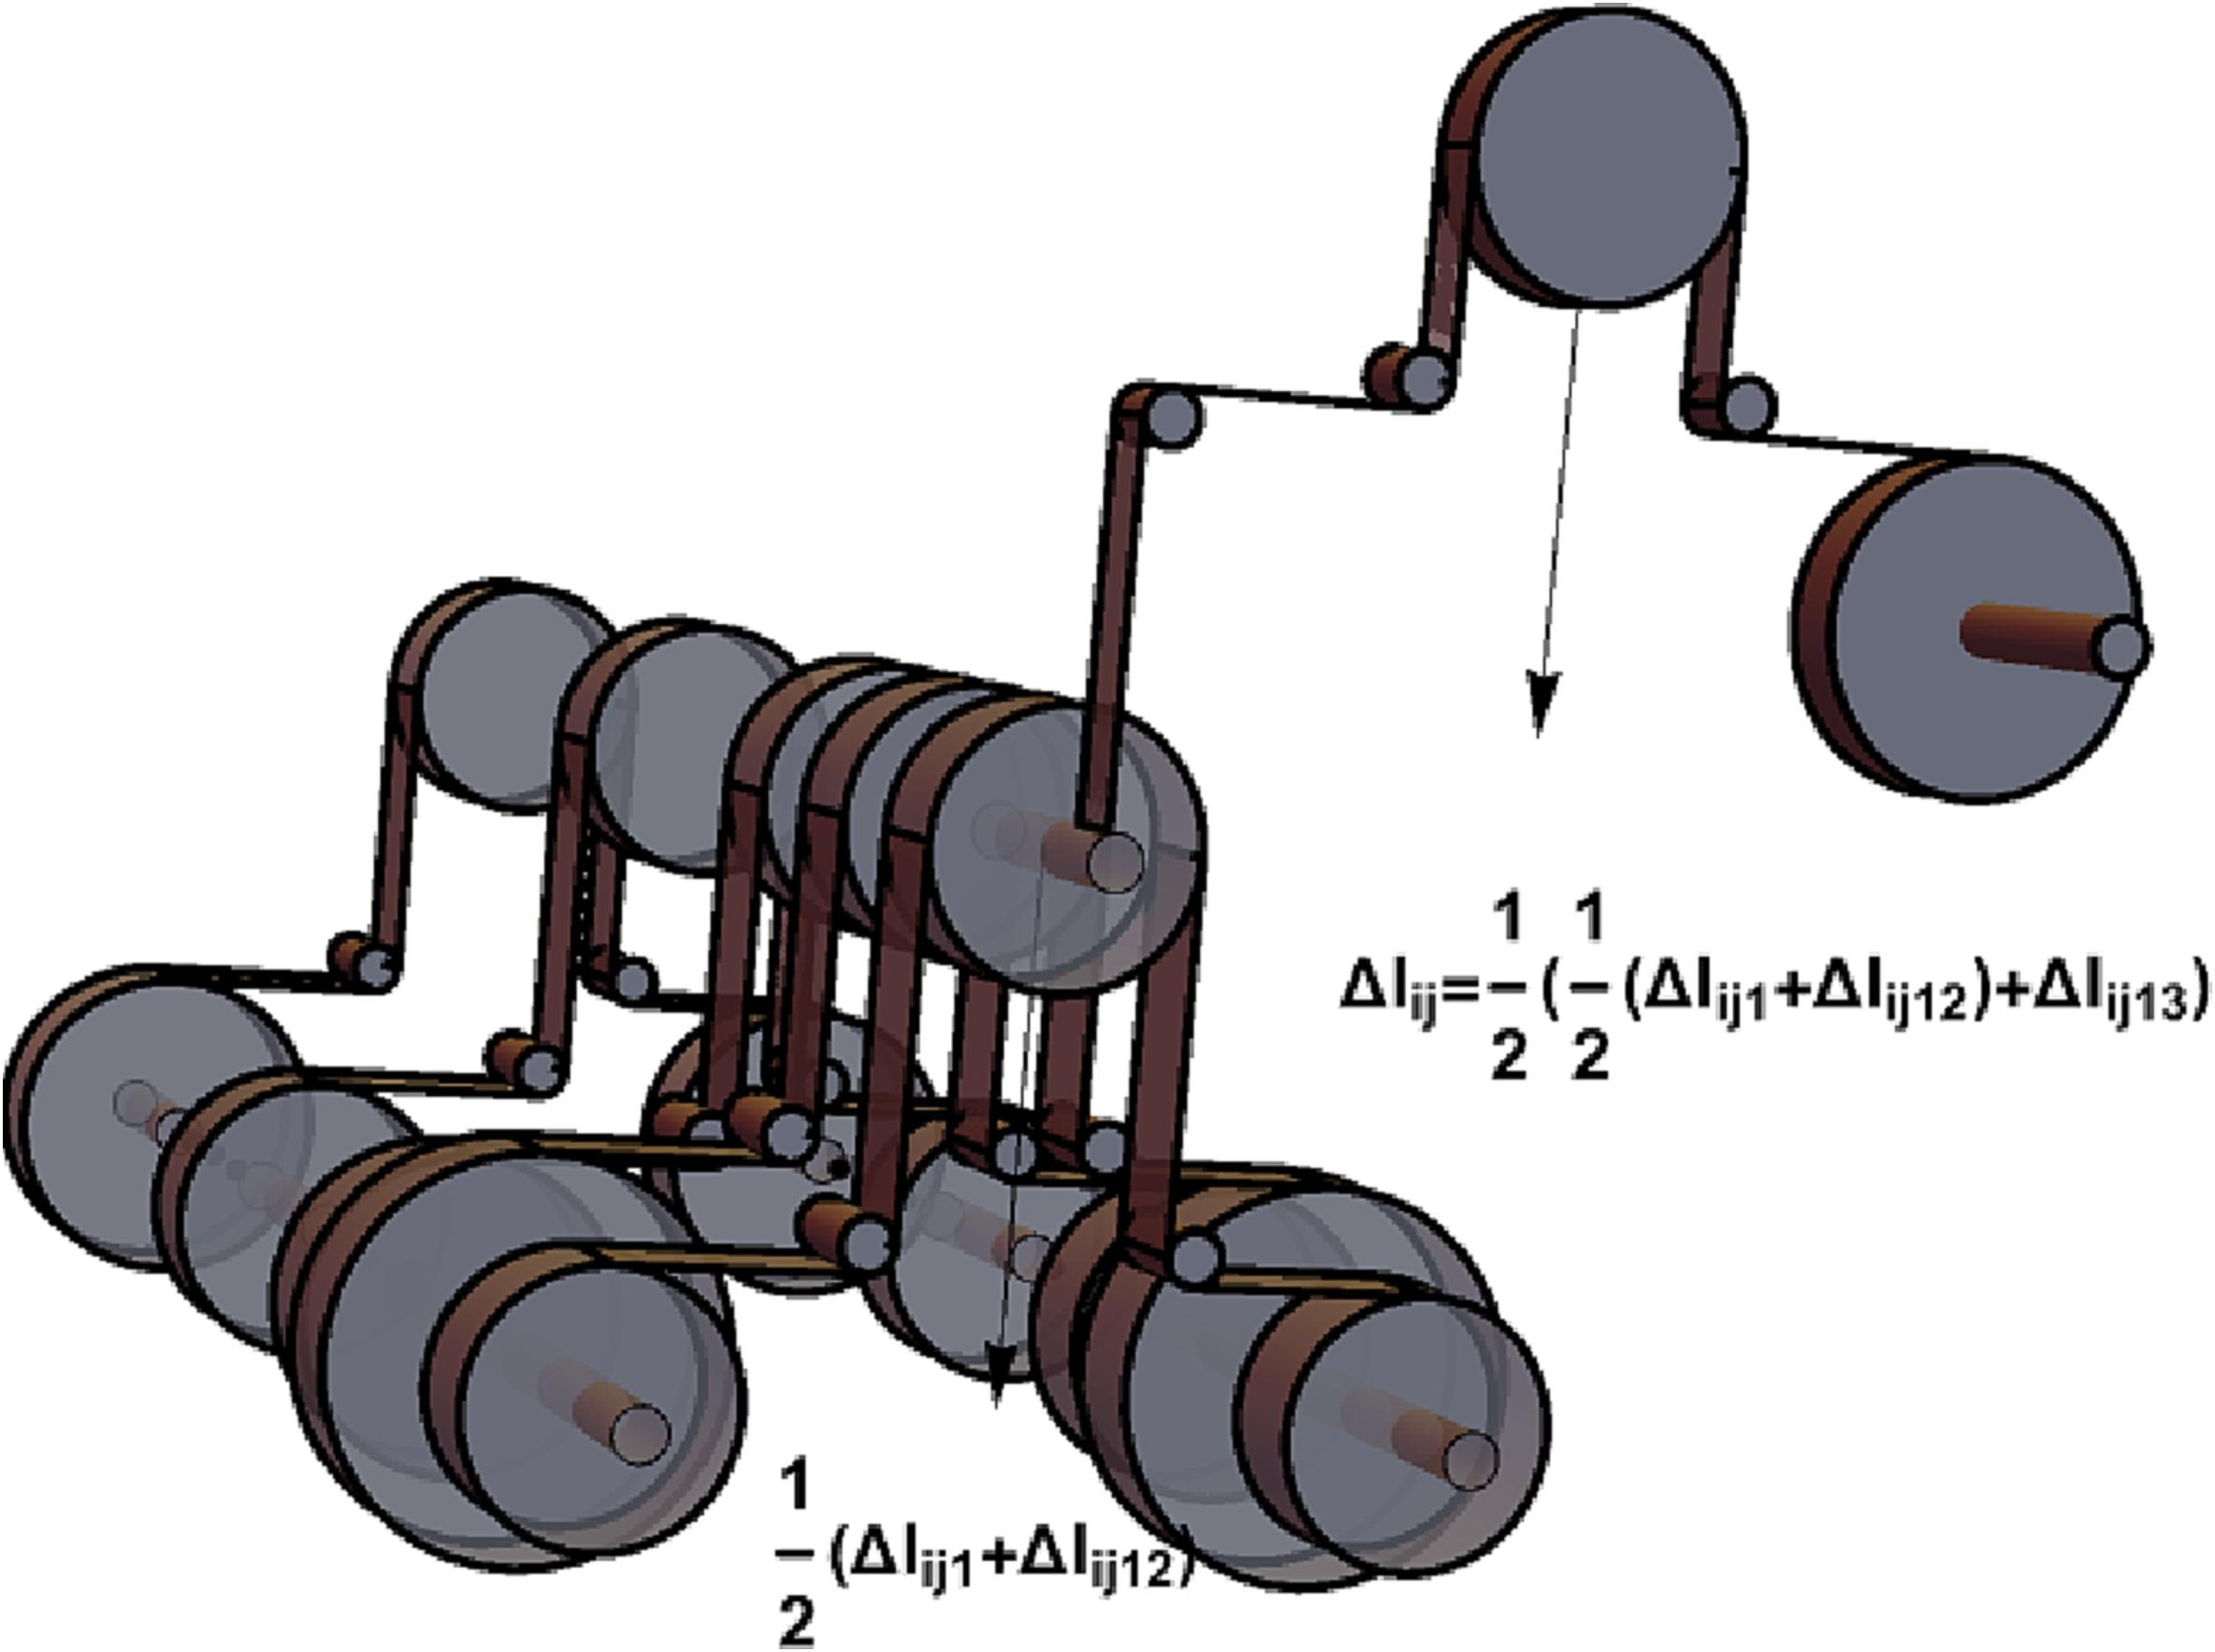
\includegraphics[width=0.5\textwidth]{Figures/poulies.jpg}
                \caption{Système de poulies pour contrôler l'exosuit. $\Delta l_{ijk}$ désigne la variation de longueur à l'instant i du câble qui, provenant de l'actionneur k, contribue au mouvement agissant sur l'articulation j \cite{daniel_rodriguez-jorge_transmission_2023}}
                \label{fig:poulies}
            \end{figure}

            L'étude \cite{daniel_rodriguez-jorge_transmission_2023} se concentre sur la conception d'exosuits à actionnement par câble pour l'assistance à la marche, une alternative aux exosquelettes rigides traditionnels. Les exosuits offrent une meilleure compatibilité cinématique avec les mouvements naturels de l'utilisateur, et sont moins chers, car ils utilisent moins d'actionneurs, notamment grâce à l'ACP (Analyse en Composantes Principales), méthode permettant d'effectuer uniquement les mouvements les plus importants. Ils utilisent en outre le principe de synergies, qui définissent un ensemble de mouvement pour prendre différents objets.

            Cette étude est intéressante pour le rôle que jouent les poulies. Ces dernières transmettent le mouvement et la force d'un actionneur (moteur dans le sac à dos) aux câbles connectés à des points d'ancrage près des articulations (hanche, genou, cheville). Leur fonction principale est de contrôler l'extension des câbles pour générer les mouvements nécessaires à l'assistance de la marche. En d'autres termes, les poulies convertissent la rotation du moteur en un déplacement linéaire des câbles, qui appliquent des forces aux points d'ancrage pour produire un couple d'assistance sur les articulations (voir figure \ref{fig:poulies}).

            Le principal inconvénient est que, si un seul actionneur ne suffit pas (par exemple, pour une précision accrue ou des besoins spécifiques), le système de transmission peut devenir très complexe et augmenter grandement les coûts de fabrication \cite{daniel_rodriguez-jorge_transmission_2023}.
            
            Dans notre cas, nous n'aurons bien qu'un seul moteur, donc nous pouvons considérer les poulies comme une solution fiable et réaliste.

        \subsubsection{Mécanisme à tendons permettant la prétension}

            Dans l'article \cite{saputro_investigation_2023}, les auteurs effectue un examen systématique de certaines avancées technologiques récentes dans le domaine des préhenseurs robotiques souples, et plus précisément dans le cas des mécanismes à tendon.

            \begin{figure}
                \centering
                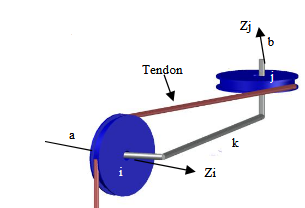
\includegraphics[width=0.7\textwidth]{Figures/tendon.png}
                \caption{Tendon à extrémité ouverte \cite{saputro_investigation_2023}}
                \label{fig:tendon}
            \end{figure}

            Une partie intéressante de cette étude est celle qui traite des tendons à extrémité ouverte, car ils permettent de prétendre le fil. Un tendon à extrémité ouverte possède une extrémité attachée à un lien mobile et l'autre extrémité fixée à une poulie motrice qui est connectée à un actionneur (notre moteur). Ce type de tendon utilise une force unidirectionnelle, la force de friction, qui agit à l'opposé de la force appliquée pour résister au mouvement du corps. Sur la figure \ref{fig:tendon}, deux poulies (i et j) sont connectées par un tendon à extrémité ouverte. Un support ou lien (noté k) est utilisé pour maintenir une distance centrale stable entre les poulies i et j. \cite{saputro_investigation_2023}

        \subsubsection{Mécanisme \textit{level wind} ou tambour}

            \begin{figure}[htbp]
                \centering
                \begin{subfigure}[t]{0.6\textwidth}
                    \centering
                    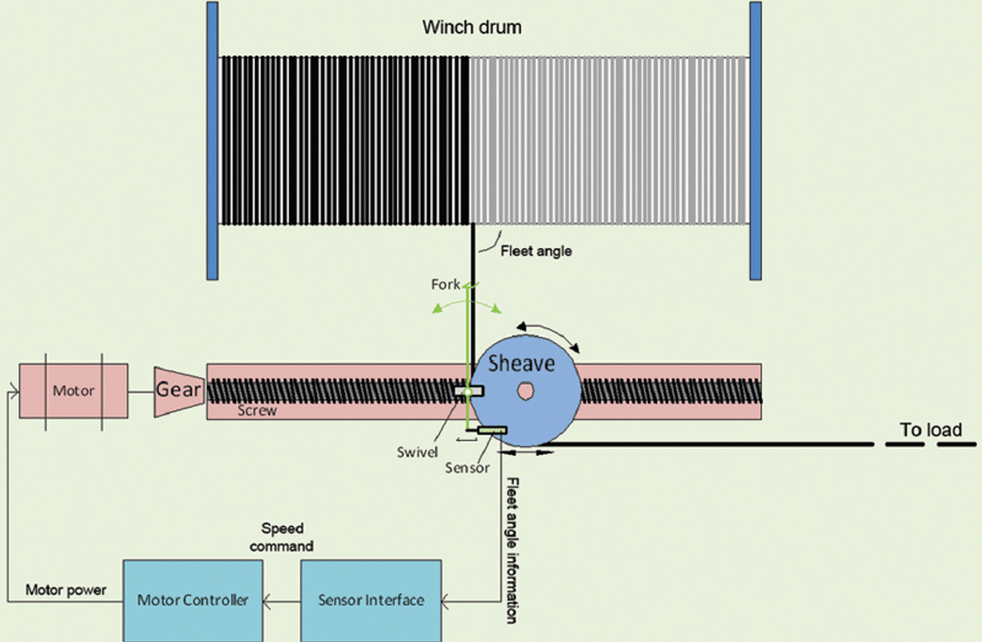
\includegraphics[width=\textwidth]{Figures/level_wind.png}
                    \caption{Principe de fonctionnement du système type \textit{level wind} \cite{mortensen_precision_2014}}
                    \label{fig:level_wind}
                \end{subfigure}
                \hfill
                \begin{subfigure}[t]{0.3\textwidth}
                    \centering
                    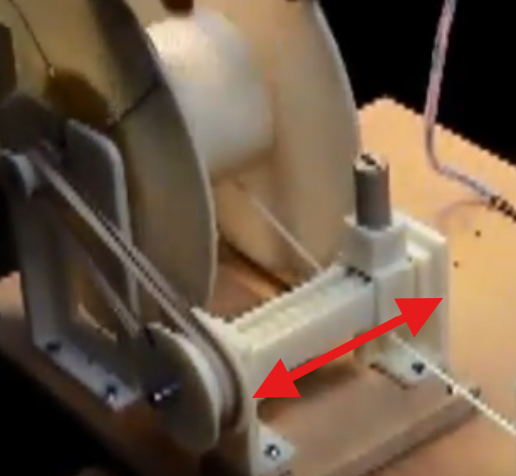
\includegraphics[width=\textwidth]{Figures/video.png}
                    \caption{Illustration du mécanisme d'enroulement \cite{hugh_lyman_level_2014}}
                    \label{fig:video}
                \end{subfigure}
                \caption{Représentation du mécanisme \textit{level wind}}
            \end{figure}

            Le mécanisme \textit{level wind} est un dispositif utilisé notamment sur les moulinets de pêche, qui guide le fil de pêche latéralement pendant l’enroulement pour éviter les enchevêtrements et maintenir une tension constante. La vidéo \cite{hugh_lyman_level_2014} illustre ce mécanisme (voir figure \ref{fig:video}).

            L'étude \cite{mortensen_precision_2014} propose un mécanisme de guidage de câble (level wind) destiné à des applications de forage profond dans la glace. Ce système assure l'enroulement uniforme du câble autour d'un tambour, tout en maintenant une tension constante, ce qui est essentiel pour éviter les erreurs de mesure et les défaillances mécaniques.

            Sur la figure \ref{fig:level_wind}, vous pouvez voir comment fonctionne le système. Une poulie se déplace le long d'un axe grâce à un moteur et une vis, et enroule alors le fil tout le long du tambour. L'approche la plus répandue pour la conception d'un tel système consiste en un rapport d'engrenage fixe entre la rotation du tambour du treuil et la poulie de l'enrouleur de niveau. Un rapport fixe signifie que pour chaque tour complet du tambour, la poulie se déplace d'une distance constante. En somme, cela permet à la poulie de se déplacer horizontalement à une vitesse proportionnelle à la vitesse de rotation du tambour. Une autre méthode, similaire à la précédente, applique ce rapport d'engrenage fixe mais est complétée par de l'automatique. Ici, la poulie est entraînée par un moteur distinct de celui du tambour. La vitesse de ce moteur est précisément synchronisée avec celle du tambour du treuil grâce à un capteur et un système de contrôle moteur en boucle fermée. \cite{mortensen_precision_2014}

            Bien que ces approches se soient révélées efficaces dans de nombreuses applications, les deux dernières conceptions sont particulièrement sensibles aux changements des conditions de fonctionnement (par exemple, la charge du câble, la température, la tolérance du capteur, la précision du calcul et l'usure des pièces mécaniques). Tout décalage entre les vitesses de rotation et les vitesses horizontales entraînait une accumulation progressive d'erreurs dans la position de la poulie par rapport au point d'entrée du câble sur le tambour du treuil. \cite{mortensen_precision_2014}

            Dans notre cas, il sera question d'un fil court et de vitesses lentes, limitant ainsi toute accumulation d'erreur dans la position de la poulie par rapport au tambour.

        \subsubsection{Vis sans fin}

            \dots

    \subsection{Simulation par éléments finis}
    
        Troisèmement, nous étudions le cas d'une simulation d'un doigt robotique qui présente de nombreuses similitudes au nôtre.
        
        \subsubsection{Étude d'un doigt pneumatique souple et simulation par éléments finis}

            \begin{figure}
                \centering
                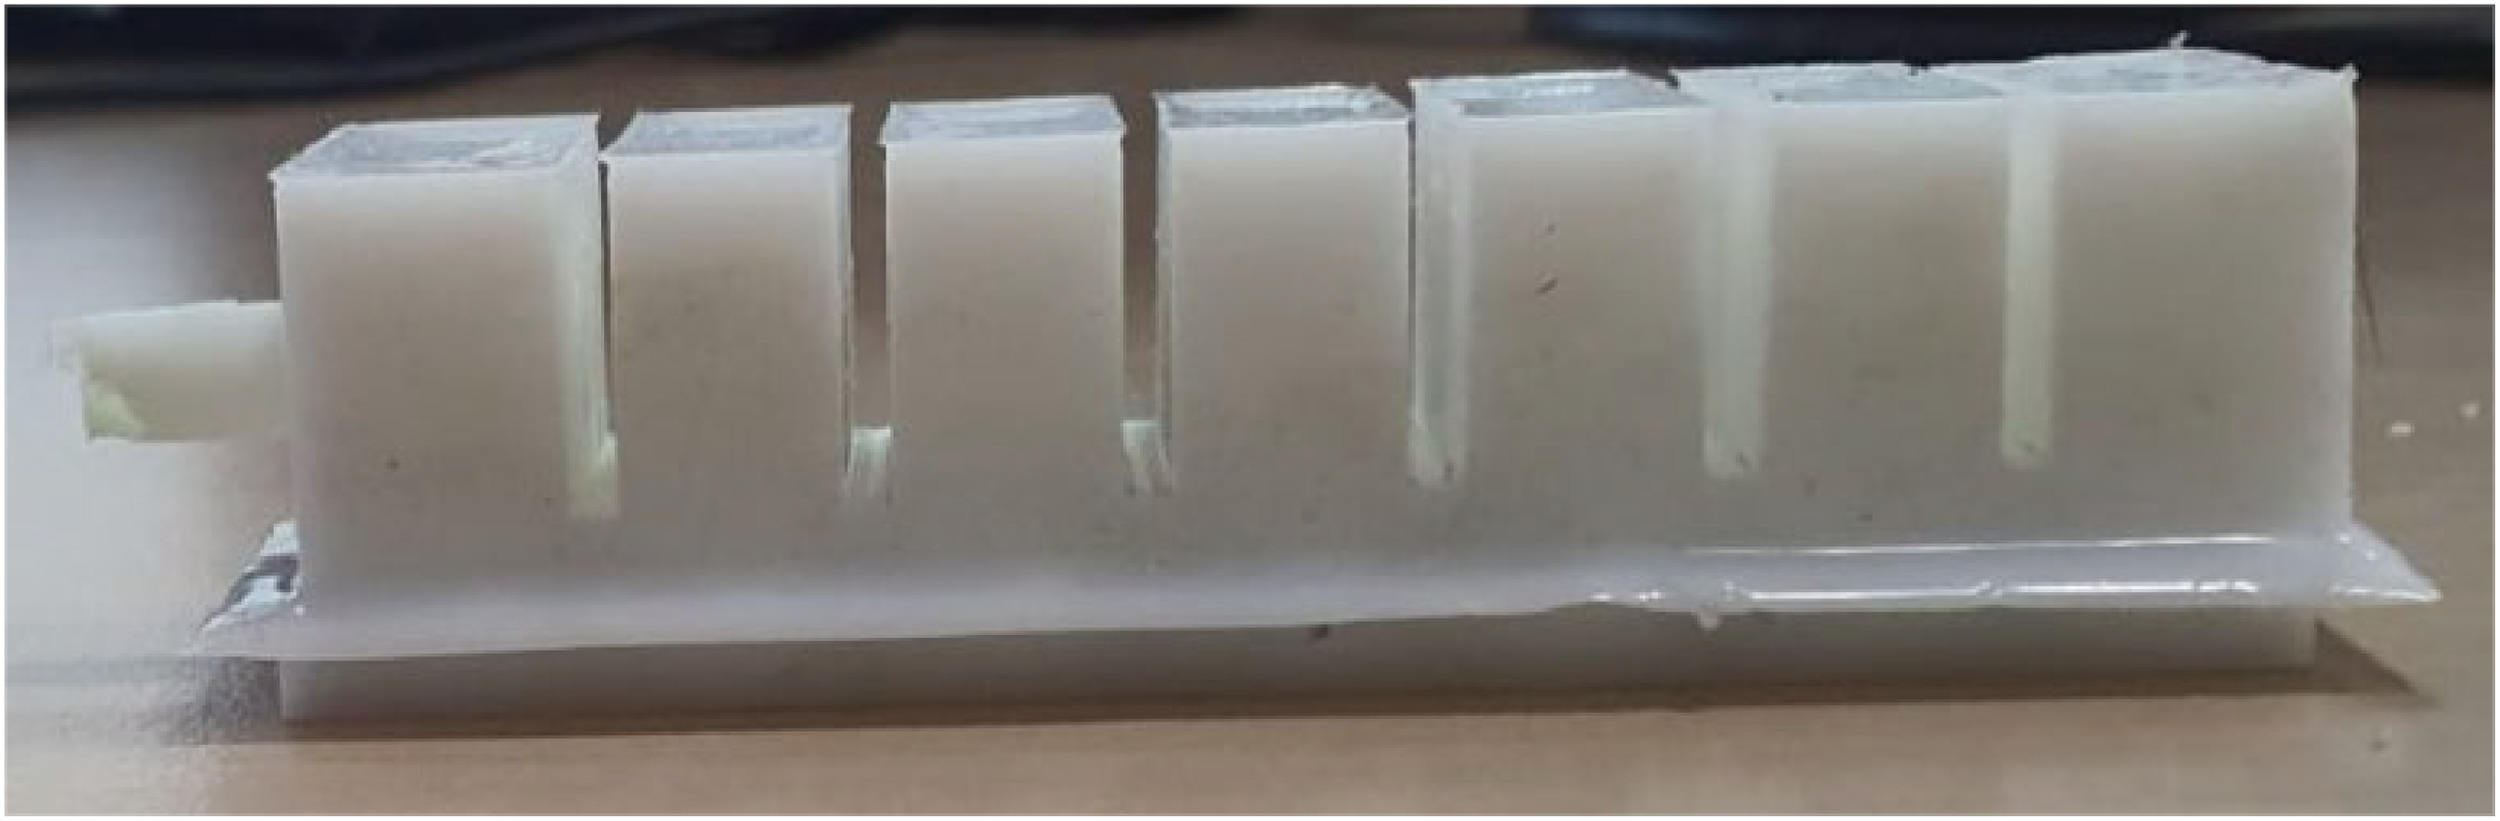
\includegraphics[width=0.7\textwidth]{Figures/doigt_souple.jpg}
                \caption{Doigt souple inspiré d'un humain \cite{bhat_numerical_2025}}
                \label{fig:doigt_souple}
            \end{figure}

            Dans \cite{bhat_numerical_2025}, les auteurs développent un actuateur souple pneumatique bio-inspiré, conçu pour la préhension douce et les applications thérapeutiques. Ce dispositif imite la flexion d’un doigt humain par l'action de la pression sur des chambres internes segmentées (voir figure \ref{fig:doigt_souple}).

            L'effecteur est fabriqué en silicone liquide (LSR), un matériau hyperélastique modélisé selon la loi de \textbf{Yeoh d'ordre 2}, adaptée aux grandes déformations quasi-incompressibles. Le modèle est défini par l'énergie de déformation suivante :

            \[
            W = \sum_{i=1}^{2} C_i (I_1 - 3)^i + D
            \]

            où :
            \begin{itemize}
            \item \( W \) est l'énergie de déformation,
            \item \( I_1 \) est le premier invariant du tenseur de Cauchy-Green à droite,
            \item \( C_1 = 0.11\,\text{MPa},\; C_2 = 0.03\,\text{MPa} \) sont les constantes matériau,
            \item le terme volumique est négligé ( \( D = 0 \) ).
            \end{itemize}

            C'est en fait la formulation faible du problème établi à l'aide du principe des travaux virtuels de l'équation de Navier-Cauchy :

            \[
            div(\sigma) + \rho f = 0
            \]

            où :
            \begin{itemize}
            \item \( \sigma \) est le tenseur de contrainte,
            \item \( \rho \) est la masse volumique,
            \item \( f \) sont les forces volumiques (gravité).
            \end{itemize}

            Le comportement est supposé \textbf{isotrope}, \textbf{homogène}, \textbf{incompressible}, et en \textbf{quasi-statique} (pas d’effets inertiels).

            \begin{figure}
                \centering
                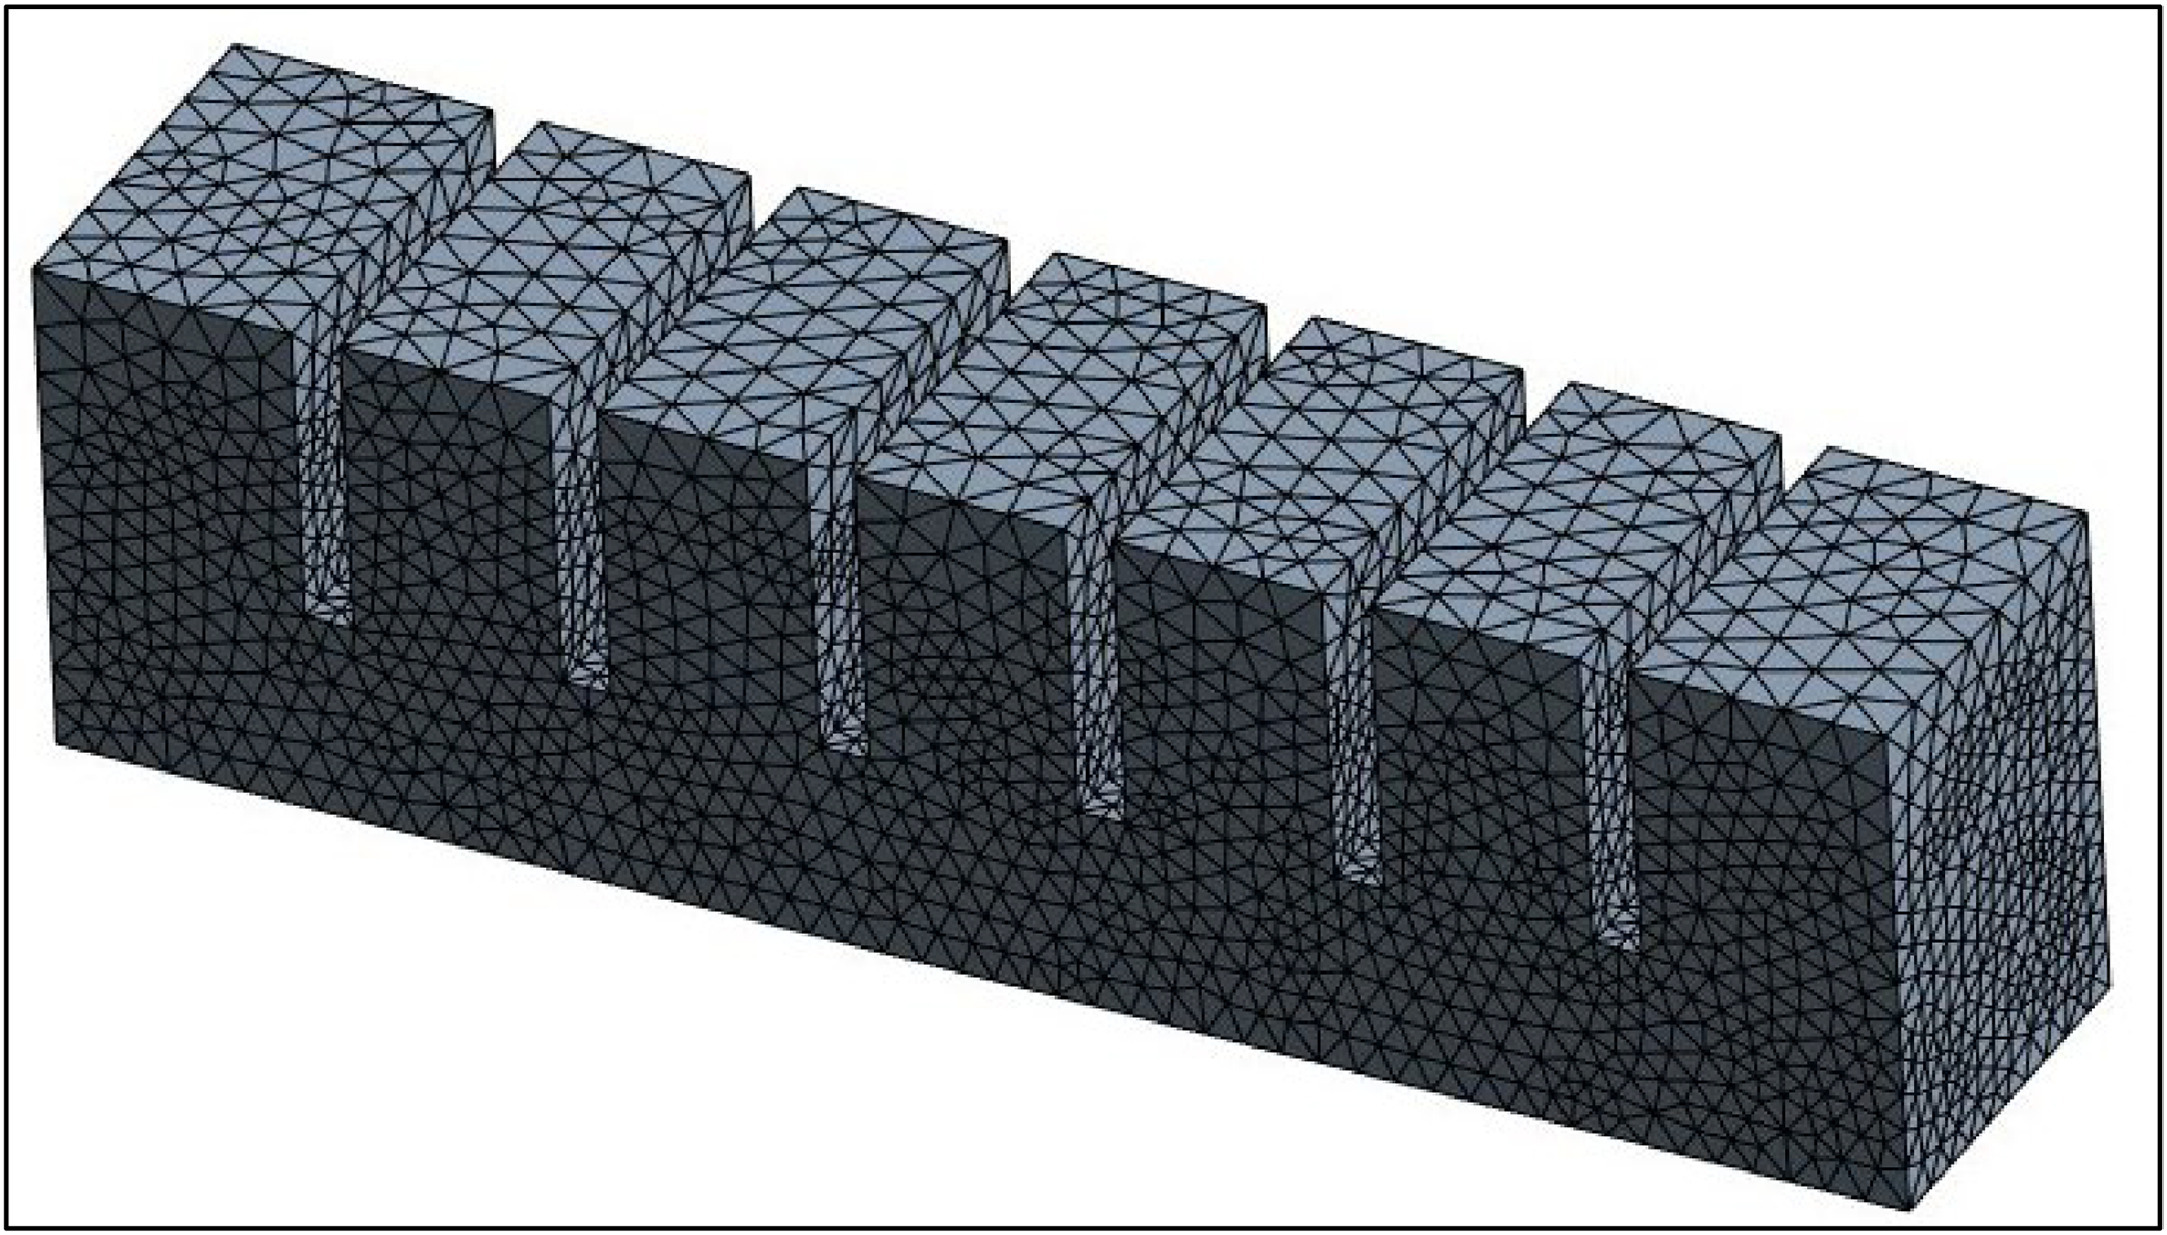
\includegraphics[width=0.7\textwidth]{Figures/doigt_finit_elements.jpg}
                \caption{Représentation du maillage du doigt \cite{bhat_numerical_2025}}
                \label{fig:doigt_finit_elements}
            \end{figure}

            L’analyse est menée via un modèle éléments finis utilisant des tétraèdres quadratiques (éléments d'ordre 2), avec un maillage raffiné (\( 63\,772 \) éléments, taille 3 mm) (voir figure \ref{fig:doigt_finit_elements}). Les conditions aux limites sont :
            \begin{itemize}
            \item Encastrement d’une extrémité de l’actuateur,
            \item Pression interne appliquée sur les parois internes,
            \item Définition de contacts sans frottement avec un bloc rigide pour calcul de la force de préhension.
            \end{itemize}

            \begin{figure}
                \centering
                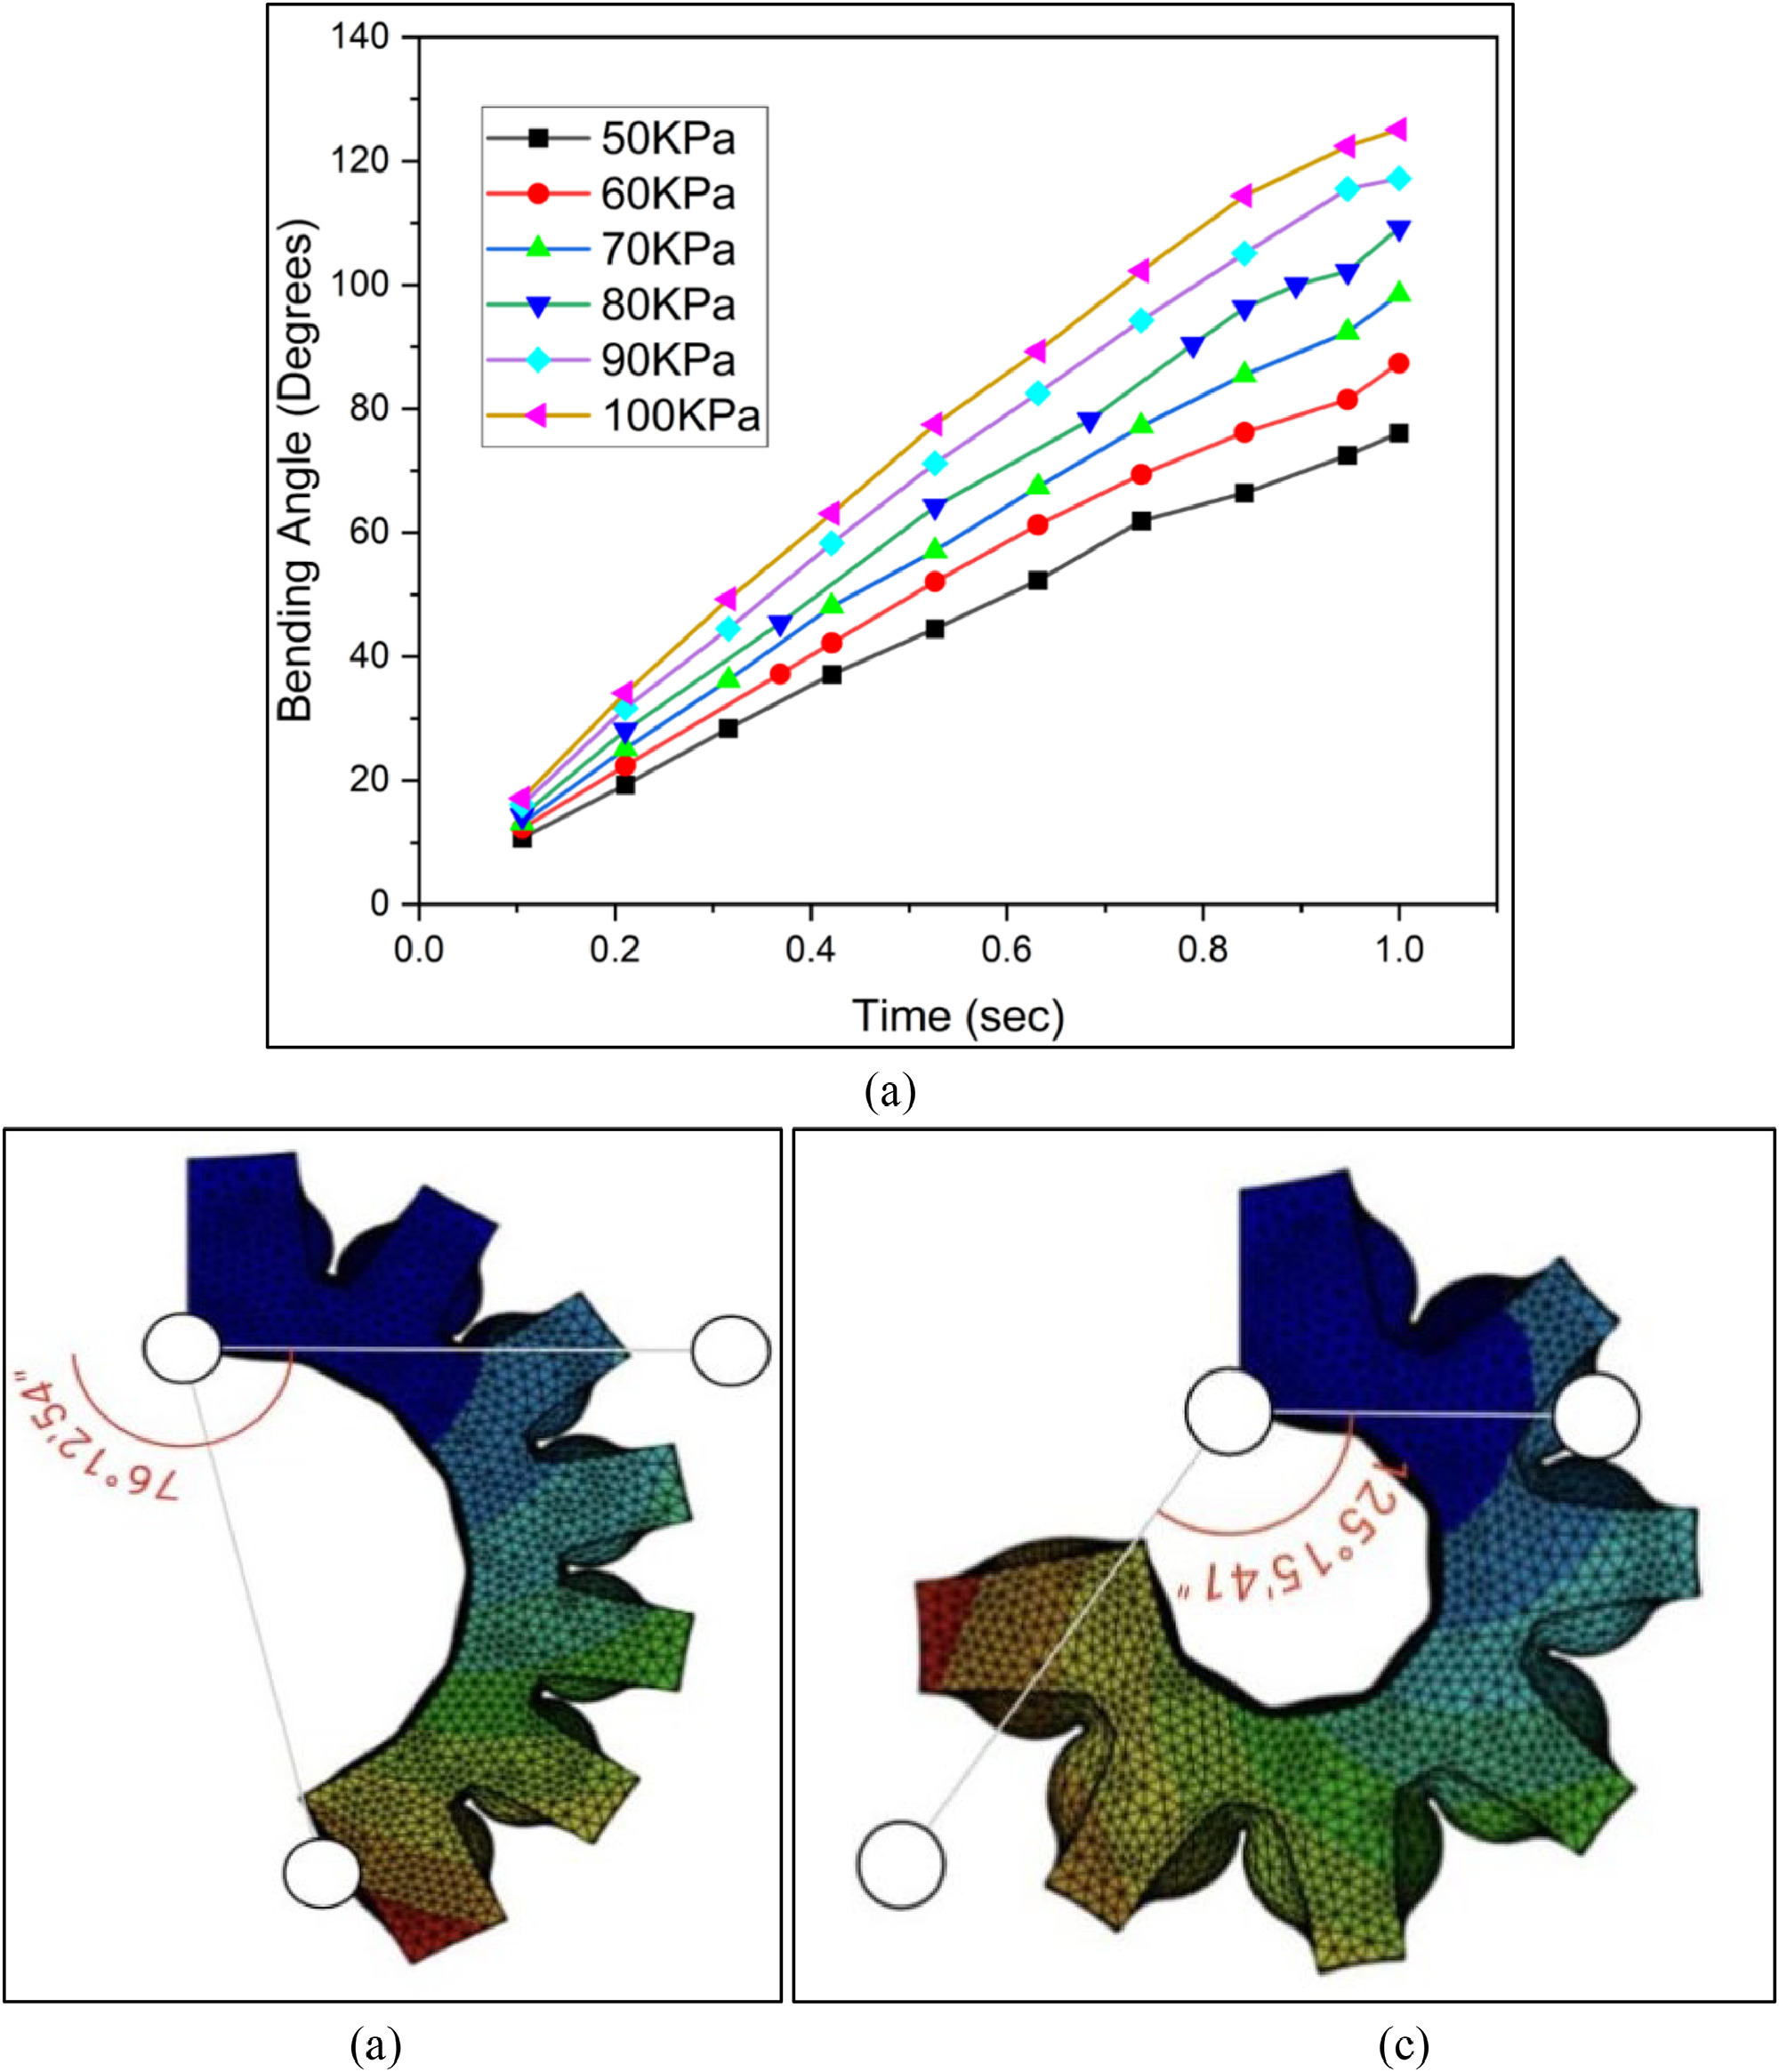
\includegraphics[width=0.6\textwidth]{Figures/angle_pression.jpg}
                \caption{Angle parcouru suivant la pression exercée (en haut), et effecteur pour une pression de respectivement de 60 kPa et 100 kPa (en bas).\cite{bhat_numerical_2025}}
                \label{fig:angle_pression}
            \end{figure}

            \begin{figure}
                \centering
                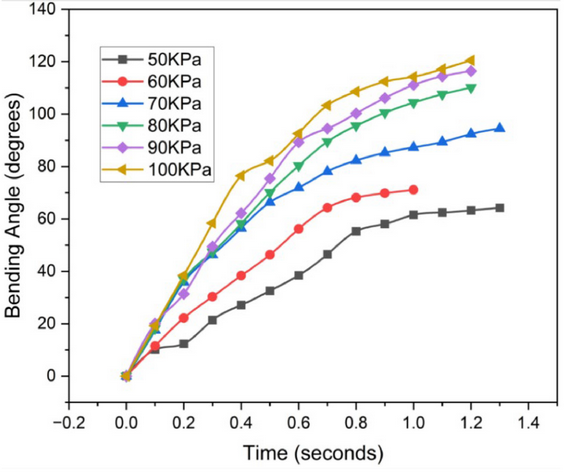
\includegraphics[width=0.6\textwidth]{Figures/angle_pression_experiments.PNG}
                \caption{Angle parcouru suivant la pression exercée lors de l'expérience \cite{bhat_numerical_2025}}
                \label{fig:angle_pression_experiments}
            \end{figure}

            L'actionneur produit une force de préhension de 2 à 2,71 N pour des pressions allant de 50 à 100 kPa, d'après la simulation. Vous pouvez trouver les résultats de sur la figure \ref{fig:angle_pression}. Lorsque l'on compare avec les données expérimentales, on n'obesrve moins cette linéarité (voir figure \ref{fig:angle_pression_experiments}). Les simulations ont également montré une force maximale de 2,71 N à 100 kPa de pression d'entrée alors que les données expérimentales obtenues par la résistance sensible à la force ont montré 5 N à 100 kPa de pression d'entrée. Ceci peut être attribué à la durée plus longue du débit d'air régulé dans l'actionneur durant les expériences par rapport aux simulations. En d'autres termes, dans les expériences pratiques, l'actionneur a eu plus de temps pour se gonfler et atteindre une force de préhension plus élevée en raison d'une alimentation en air prolongée, ce qui n'a pas été entièrement capturé ou reproduit dans les simulations. Ces résultats sont comparables à ceux rapportés pour les pinces robotisées molles dans la littérature. \cite{bhat_numerical_2025}

            Ce travail démontre qu'un actionneur pneumatique souple bien conçu peut produire des forces de préhension tout en conservant une grande capacité de déformation. Il offre une référence utile pour la conception de dispositifs bio-inspirés, bien que son mode d'action pneumatique diffère de notre approche par câbles, qui est plus compacte pour un système embarqué. Cet article nous a néanmoins permis d'explorer un exemple de modèle de déformation et nous a fourni une première perspective pour la mise en place d'une simulation utilisant un maillage fin via un modèle CAO.
    
    \subsection{Conclusion}

        En somme, les approches existantes confirment l’intérêt des structures souples et des actionnements par câble pour des tâches de préhension adaptative. Toutefois, elles soulignent aussi les limites à surmonter, notamment en matière de charge maximale, de précision et de contrôle de la tension. Ces constats guideront nos choix dans la conception de la pince proposée.

\clearpage
        
\section{Conception de la pince}
        
    \subsection{Considérations mathématiques}

        \textcolor{red}{Modifie selon ce que tu as fais}

        \textcolor{red}{Les valeurs de $\theta_0$ sont à modifier !!!}

        \subsubsection{Spirale centrale}
            
            Sur la figure \ref{fig:spiral_logarithm}, la spirale centrale (en orange) qui définit notre robot vérifie la relation :
            \begin{equation}
            r_c(\theta) = \frac{r(\theta) + r(\theta + 2\pi)}{2}, \quad \forall \theta
            \label{eq:spirale_centrale}
            \end{equation}
            
            Cela signifie qu’on prend le rayon de la spirale du robot (en noire) au point $\theta$ ($r(\theta)$), et au point $\theta + 2\pi$ ($r(\theta + 2\pi)$), et on calcule leur moyenne. Cela donne un point « central » pour chaque angle $\theta$, et en les reliant, on forme la spirale centrale. \cite{wang_spirobs_2025}

        \subsubsection{Choix et détermination des coefficients}

            \begin{figure}
                \centering
                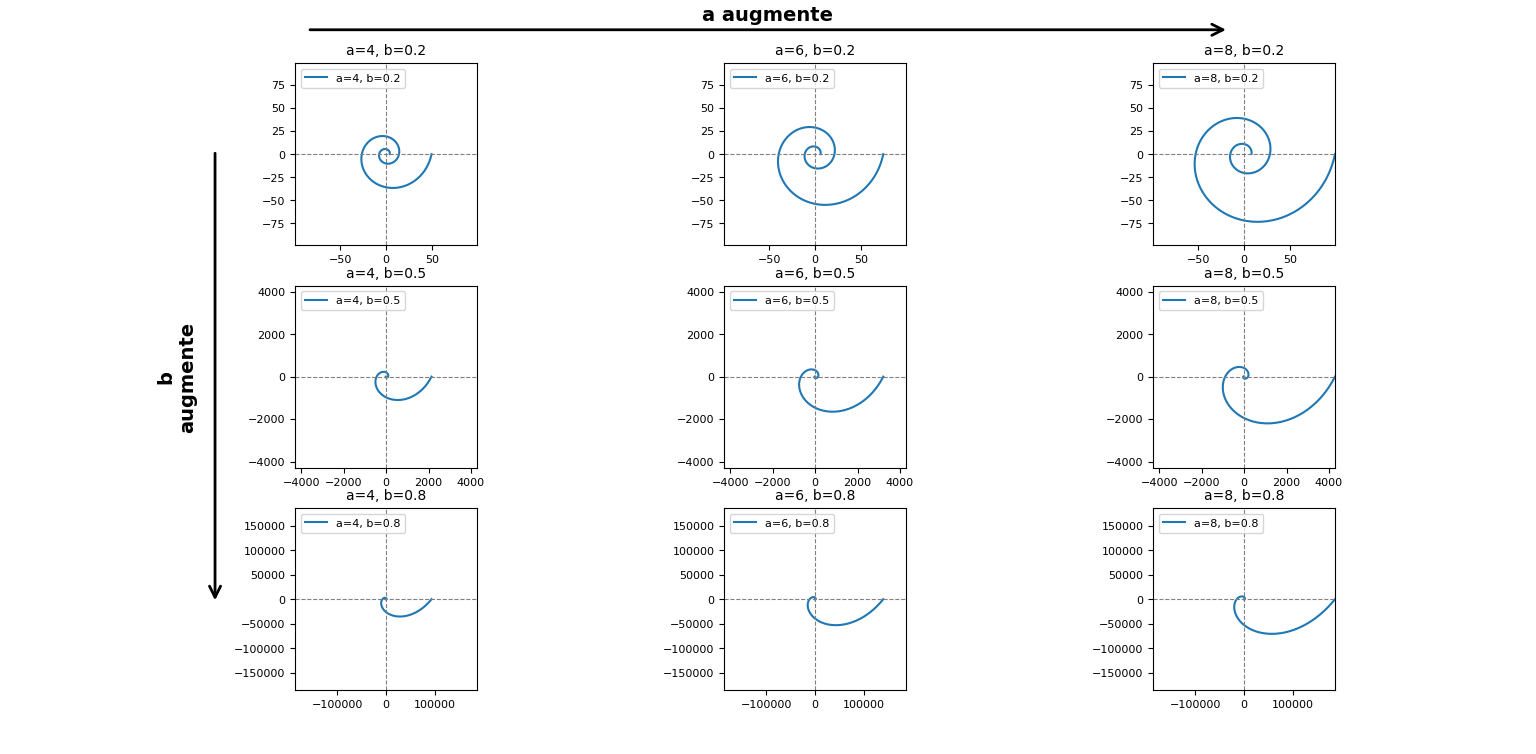
\includegraphics[width=1\textwidth]{Figures/spirale.png}
                \caption{Influence des coefficients $a$ et $b$ sur le tracé de la spirale logarithmique}
                \label{fig:spirale}
            \end{figure}
        
            Dans \cite{wang_spirobs_2025}, les auteurs expliquent comment dessiner le SpiRob. Nous nous inspirons de sa forme pour concevoir nos doigts.
        
            La spirale logarithmique est d'équation en coordonnées polaires ($r, \theta$) :

            \begin{equation}
                r = ae^{b\theta}, \quad \text{avec} \quad a > 0
                \label{eq:spirale_log}
            \end{equation}
            
            Sachant que $a$ est un paramètre d’échelle (elle détermine la taille globale de la spirale). Tandis que $b$ est un autre paramètre d’échelle qui détermine à quel point la spirale s’enroule (plus $b$ est grand, plus la spirale est "serrée"), comme l'illustre la figure \ref{fig:spirale}.
            
            Idéalement, nous aurons besoin que la spirale s'enroule complètement autour de l'objet pour le saisir, donc nous utiliserons un $b$ relativement petit, $a$ sera choisi de telle sorte que la spirale déroulée mesurera 10 cm, tandis que la spirale parcourra 1 tour complet.
        
            Pour déterminer la valeur de \( a \) dans l'équation de la spirale logarithmique \( r = a \cdot e^{b \cdot \theta} \), où la longueur totale déroulée \( L \) doit être égale à 100 mm, nous procédons comme suit :

            La longueur totale \( L \) d'une spirale logarithmique est donnée par l'intégrale de l'arc de $0$ à $2\pi$ :
            \[
            L = \int_0^{\theta_0} \sqrt{r^2 + \left(\frac{dr}{d\theta}\right)^2} \, d\theta, \, \text{pour} \, \theta_0 = 2\pi \, \text{(1 tour complet)}
            \]

            \textcolor{red}{$\theta_0 = \frac{3\pi}{2}$ au lieu de $2\pi$ !!!}
            
            Calculons la dérivée de \( r \) par rapport à \( \theta \) :
            \[
            \frac{dr}{d\theta} = \frac{d}{d\theta} \left( a \cdot e^{b \cdot \theta} \right) = a \cdot b \cdot e^{b \cdot \theta}
            \]
            
            Substituons dans l'expression sous la racine :
            \[
            r^2 = \left( a \cdot e^{b \cdot \theta} \right)^2 = a^2 \cdot e^{2b \theta}
            \]
            \[
            \left( \frac{dr}{d\theta} \right)^2 = \left( a \cdot b \cdot e^{b \cdot \theta} \right)^2 = a^2 \cdot b^2 \cdot e^{2b \theta}
            \]
            \[
            r^2 + \left( \frac{dr}{d\theta} \right)^2 = a^2 e^{2b \theta} + a^2 b^2 e^{2b \theta} = a^2 e^{2b \theta} (1 + b^2)
            \]
            
            Prenons la racine carrée :
            \[
            \sqrt{r^2 + \left( \frac{dr}{d\theta} \right)^2} = \sqrt{a^2 e^{2b \theta} (1 + b^2)} = a e^{b \theta} \sqrt{1 + b^2}
            \]
            
            La longueur totale devient :
            \[
            L = \int_0^{2\pi} a e^{b \theta} \sqrt{1 + b^2} \, d\theta = a \sqrt{1 + b^2} \int_0^{2\pi} e^{b \theta} \, d\theta
            \]
            
            Calculons l'intégrale :
            \[
            \int_0^{2\pi} e^{b \theta} \, d\theta = \left[ \frac{1}{b} e^{b \theta} \right]_0^{2\pi} = \frac{1}{b} \left( e^{b \cdot 2\pi} - e^{b \cdot 0} \right) = \frac{1}{b} \left( e^{b \cdot 2\pi} - 1 \right)
            \]
            
            Ainsi, la longueur totale est :
            \[
            L = a \sqrt{1 + b^2} \cdot \frac{1}{b} \left( e^{b \cdot 2\pi} - 1 \right)
            \]
            
            En isolant \( a \) :
            \[
            a = \frac{L}{\sqrt{1 + b^2} \cdot \frac{1}{b} \left( e^{b \cdot 2\pi} - 1 \right)} = \frac{L b}{\sqrt{1 + b^2} \left( e^{b \cdot 2\pi} - 1 \right)}
            \]
            
            Applications numériques avec \( b \in \{0.1, 0.2, 0.3, \dots, 1.0\} \) et \( L = 100 \) mm:

            \begin{table}[h!]
                \centering
                \begin{tabular}{@{}c S[table-format=1.4]@{}}
                \toprule
                $b$ & {$a$ [mm]} \\
                \midrule
                0.1 & 3.9557 \\
                0.2 & 1.7272 \\
                0.3 & 0.6783 \\
                0.4 & 0.2460 \\
                0.5 & 0.0837 \\
                0.6 & 0.0273 \\
                0.7 & 0.0087 \\
                0.8 & 0.0027 \\
                0.9 & 0.0008 \\
                1.0 & 0.0002 \\
                \bottomrule
                \end{tabular}
                \caption{Valeurs de $a$ calculées pour différentes valeurs de $b$ avec $L=100$ mm.}
            \end{table}

        \subsubsection{Espacement}
            
            Enfin, il reste l'espacement $\Delta\theta$ à choisir entre les unités de la figure \ref{fig:spiral_logarithm} pour définir entièrement la forme et la taille du doigt. \cite{wang_spirobs_2025} Or, si $\theta$ va de $0$ à $2\pi$, le nombre de segments est :
        
            \begin{equation}
            \text{Nombre de rainures} = N = \frac{\text{Angle total}}{\Delta\theta}
            = \frac{\theta_0}{\Delta \theta}
            = \frac{2\pi}{\Delta\theta}
            \label{eq:nb_segment}
            \end{equation}

        \subsubsection{Spirale déroulée}

            \begin{figure}
                \centering
                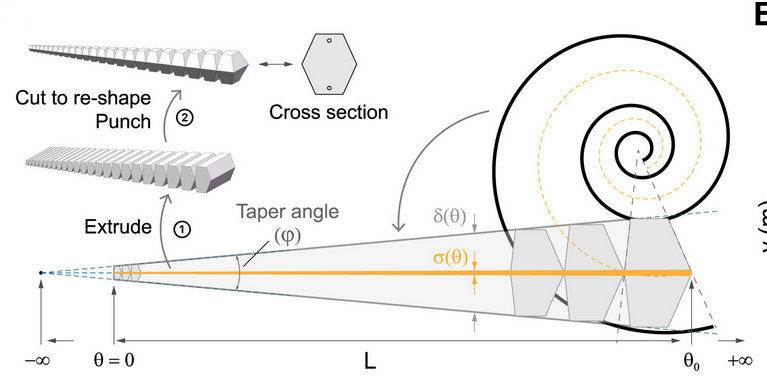
\includegraphics[width=0.7\textwidth]{Figures/draw_solidworks.png}
                \caption{Construction du doigt en "dépliant" la spirale logarthimique \cite{wang_spirobs_2025}}
                \label{fig:draw_solidworks}
            \end{figure}

            Pour dessiner le doigt sur SolidWorks, nous prenons exemple sur la figure \ref{fig:draw_solidworks}. Nous optons néanmoins pour un bossage extrudé à la place de la révolution. Il est désormais question de traduire le formalisme mathématique de la spirale logarthmique en côte des différentes rainures qui composent le doigt.

            On donne l'angle de conicité :

            \begin{equation}
            \phi = 2\arctan \left(
                \frac{\frac{1}{2}\delta(\theta)}{L(-\infty, \theta)}
                \right) = 2 \arctan\left(\frac{b(e^{2\pi b}-1)}{\sqrt{b^2+1} \left(e^{2\pi b}+1\right)}\right)
            \label{eq:angle_de_conicite}
            \end{equation}

            Avec :

            \begin{itemize}
                \item l'épaisseur du robot à l'angle $\theta$ : $\delta(\theta) = ae^{(b\theta + 2\pi)} - ae^{b\theta}$
                \item la longueur du robot entre $[-\infty,\theta]$ : $L(-\infty, \theta) = \int_{-\infty}^{\theta} \sqrt{r_c^2 + \left(\frac{dr}{d\theta}\right)^2} \, d\theta = \frac{r_c(\theta)}{b}$.
            \end{itemize}

            Le fait que $\phi$ soit indépendant de $\theta$ signifie que la forme est effilée \cite{wang_spirobs_2025}.

            Enfin, le rapport entre les épaisseurs de deux rainures adjacentes \(\beta\) est donnée par :
            \begin{equation}
            \beta = \frac{\delta(\theta + \Delta\theta)}{\delta(\theta)} = e^{b \Delta\theta}
            \label{eq:beta}
            \end{equation}
            
            Cela signifie que la taille ou la géométrie d’une rainures peut être mise à l’échelle (agrandie ou réduite) par un facteur $\beta$ par rapport à la rainure précédente. Ainsi, il suffit de concevoir une seule rainure de base, puis de l’ajuster avec $\beta$ pour créer les rainures adjacentes.

            Pour les raisons spécifiées plus tôt, nous prenons $b = 0.2$. Egalement, nous souhaitons que le nombre de rainures $N = 10$, alors, d'après (\ref{eq:nb_segment}), on a :

            \[
            \Delta\theta= \frac{\text{Angle total}}{N} = \frac{2\pi}{10} \approx 0.628 \text{ rad} \approx 36^{\circ}
            \]
            
            On calcule notre angle de conicité grâce à (\ref{eq:angle_de_conicite}) :
            
            \[
            \phi = 2 \arctan\left( \frac{0.2\left(e^{2\pi \cdot 0.2} - 1\right)}{\sqrt{0.2^2 + 1} \left(e^{2\pi \cdot 0.2} + 1\right)} \right)
            = 0.4656 \text{ rad}
            = 26.13^{\circ}
            \]

            Cela nous permet de dessiner les lignes de construction de l'enleveloppe de notre doigt. On ne dessine que d'un côté dans l'objectif de construire l'autre par symétrie.

            Par ailleurs, l'angle de conicité de la spirale joue un rôle clé dans les performances de préhension du doigt, notamment en termes d’espace de travail, de précision de saisie et de capacité de charge. 
            D’après les résultats rapportés dans \cite{wang_spirobs_2025}, un \textbf{faible angle de conicité} permet d’augmenter significativement l’espace de travail, en élargissant la zone accessible par les doigts lors du déploiement. À l’inverse, un \textbf{angle de conicité plus élevé} améliore la performance de saisie : il permet de saisir des objets de plus petite taille (diamètre minimal réduit) tout en augmentant la \textbf{capacité de charge maximale} du robot.
            À géométrie constante, l’augmentation du poids de l’objet à saisir est également mieux tolérée lorsque le diamètre est grand, ce phénomène étant particulièrement marqué pour les objets volumineux. Par exemple, un SpiRob avec un angle de conicité de $15^\circ$ peut saisir des objets dont le diamètre varie de \textbf{5{,}6\,mm à 115\,mm}, et supporter une charge allant jusqu’à \textbf{10\,kg}, soit environ \textbf{260 fois son propre poids} (poids du robot : 38{,}4\,g) \cite{wang_spirobs_2025}.

            Ainsi, comme il s'agit d'une pince attachée à un bras robotique, la pince en elle-même n'a pas besoin d'un espace de travail important, c'est pourquoi notre angle de conicité est satisfaisant pour répondre à une bonne performance de saisie.

            Il nous reste maintenant à baisser d'un rapport $\beta$ la rainure construite pour créer celle d'après... (je te laisse faire).
            
            Calculons $\beta$ grâce à (\ref{eq:beta}):

            \[
            \beta = e^{0.2 * 0.628} = 1.134
            \]

    \subsection{Dessin sur SolidWorks}

        \subsubsection{Dessin du doigt}

            \dots

        \subsubsection{Création d'un matériau TPU}

            \dots

        \subsubsection{Dessin de la base}

            \dots

        \subsubsection{Dessin de l'actionneur}

            \begin{figure}
                \centering
                \begin{subfigure}[t]{0.6\textwidth}
                    \centering
                    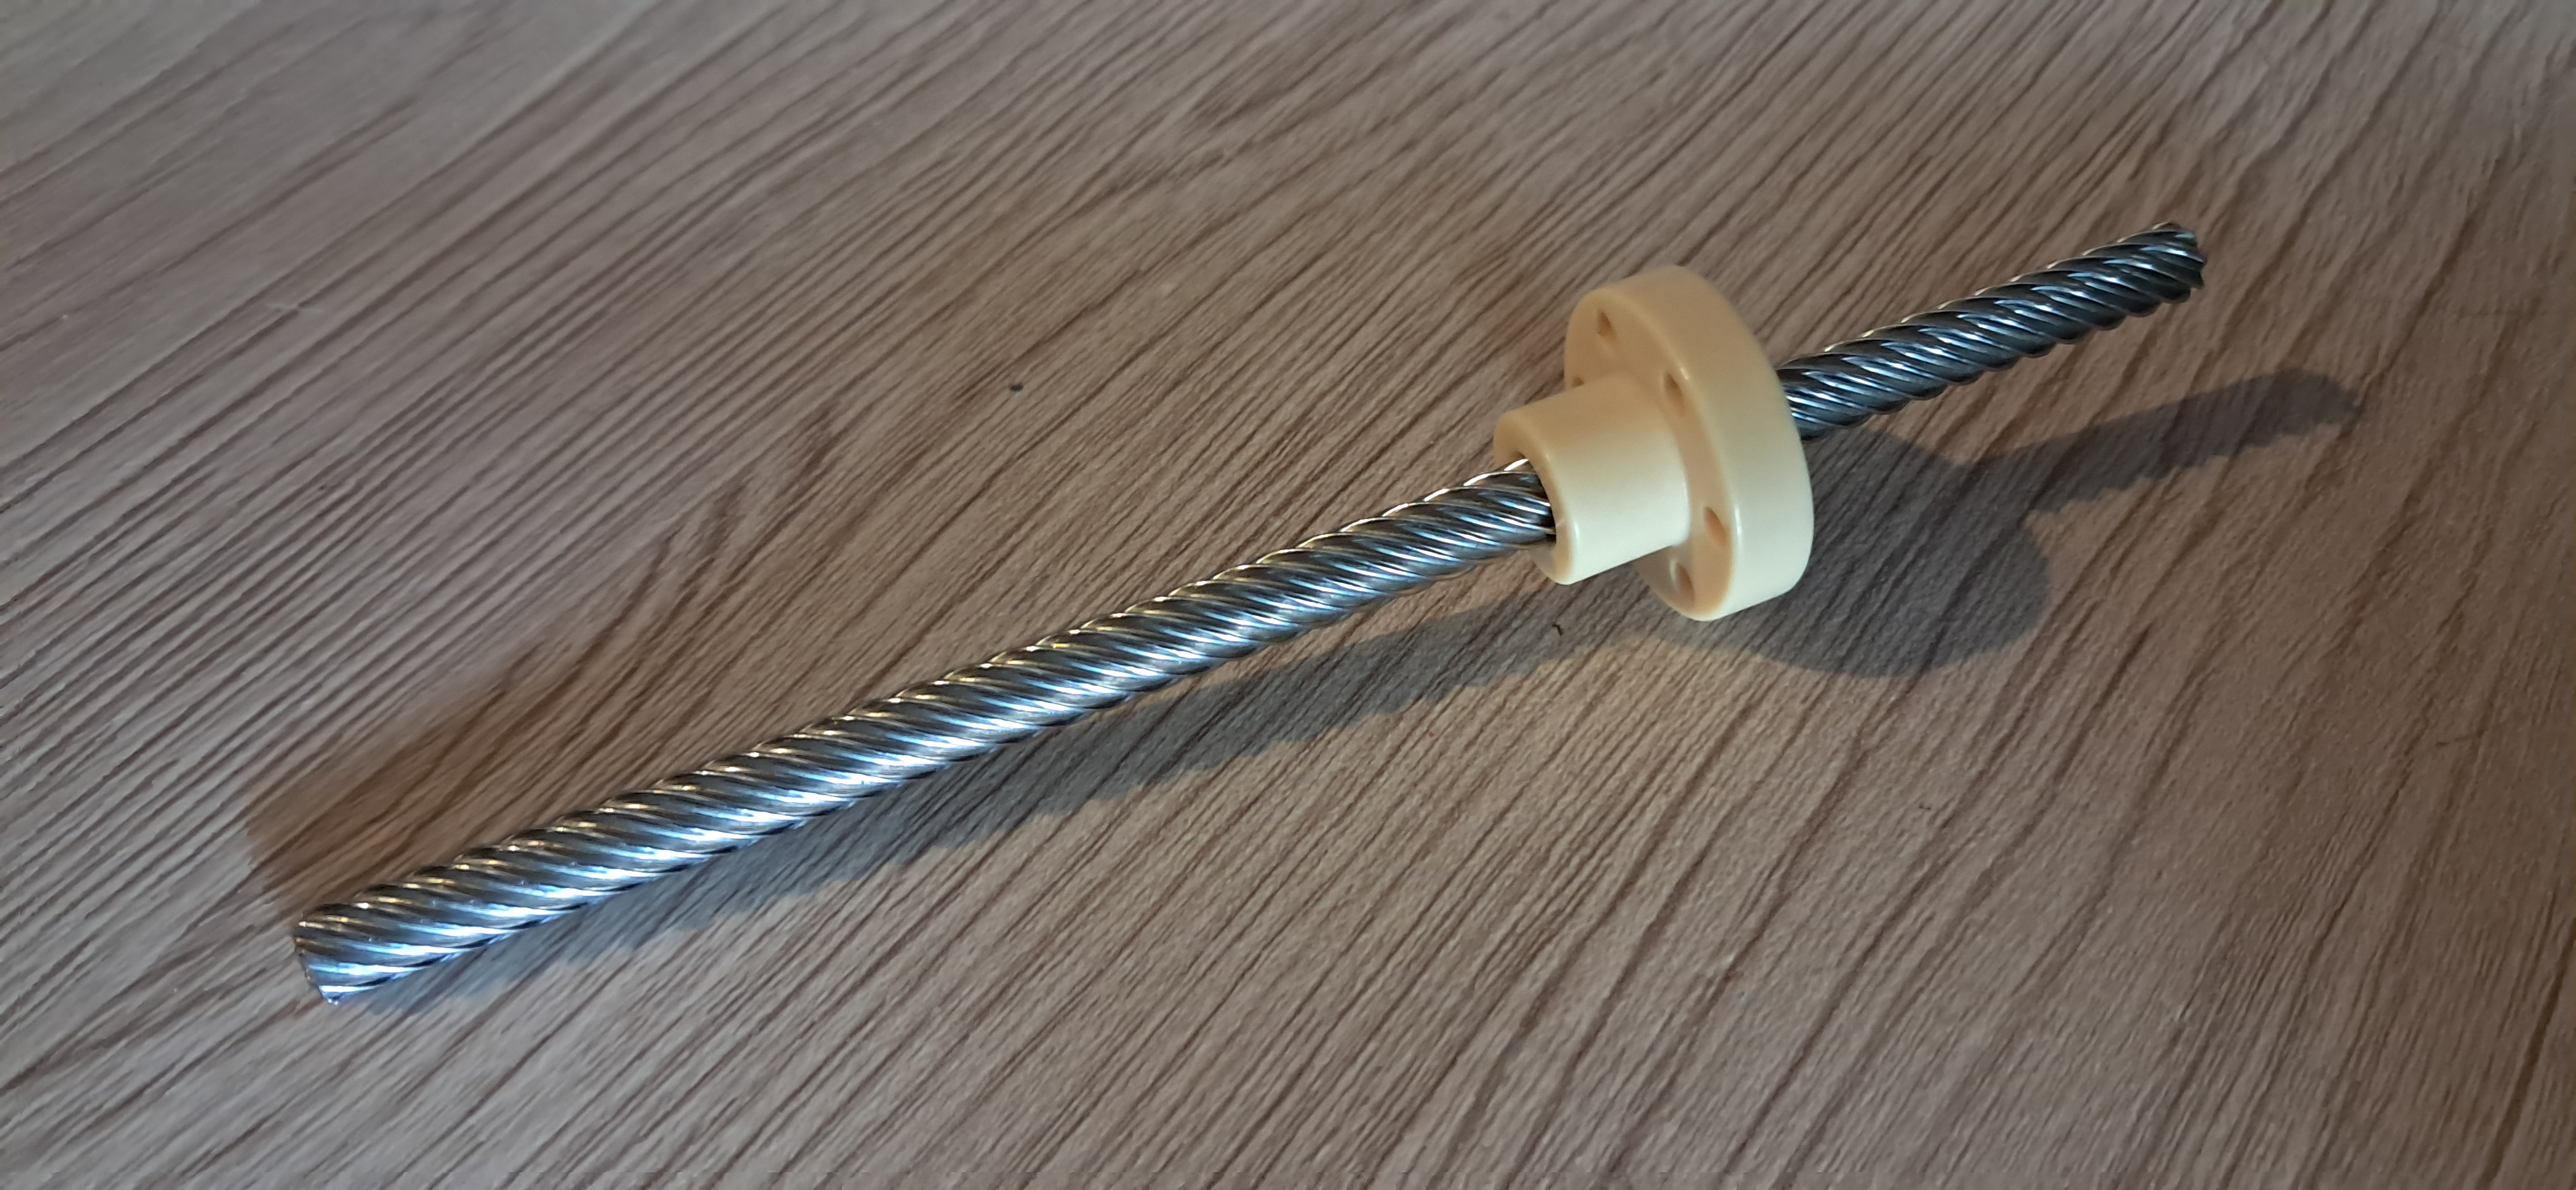
\includegraphics[width=\textwidth]{Figures/vis_sans_fin.jpg}
                    \caption{Notre vis mère de la marque Igus}
                    \label{fig:vis_sans_fin}
                \end{subfigure}
                \hfill
                \begin{subfigure}[t]{0.3\textwidth}
                    \centering
                    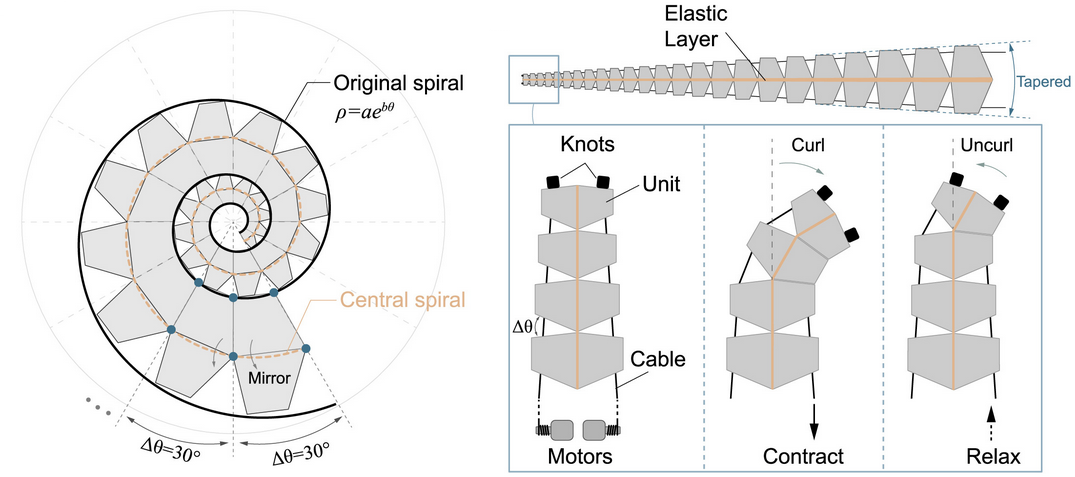
\includegraphics[width=\textwidth]{Figures/spiral_logarithm.png}
                    \caption{Modèle de la vis sans fin trouvée sur \textit{mcmaster.com}}
                    \label{fig:vis_sans_fin_solidworks}
                \end{subfigure}
                \caption{Illustrations de la vis sans fin}
            \end{figure}

            Après concertation avec notre superviseur, nous n'allons pas utiliser de tambour pour l'actionnement par câble. En effet, le tambour est une bonne solution mais la vis mère demeure davantage simple à mettre en œuvre. Dans le cadre de notre projet, nous allons donc utiliser un servomoteur et une vis mère (voir figure \ref{fig:vis_sans_fin}), qui tirera des câbles de type UHMWPE, car ces derniers possèdent un faible coefficient de frottement et une importante résistance à l'usure \cite{wang_spirobs_2025}.

            \begin{figure}
                \centering
                \begin{subfigure}[t]{0.5\textwidth}
                    \centering
                    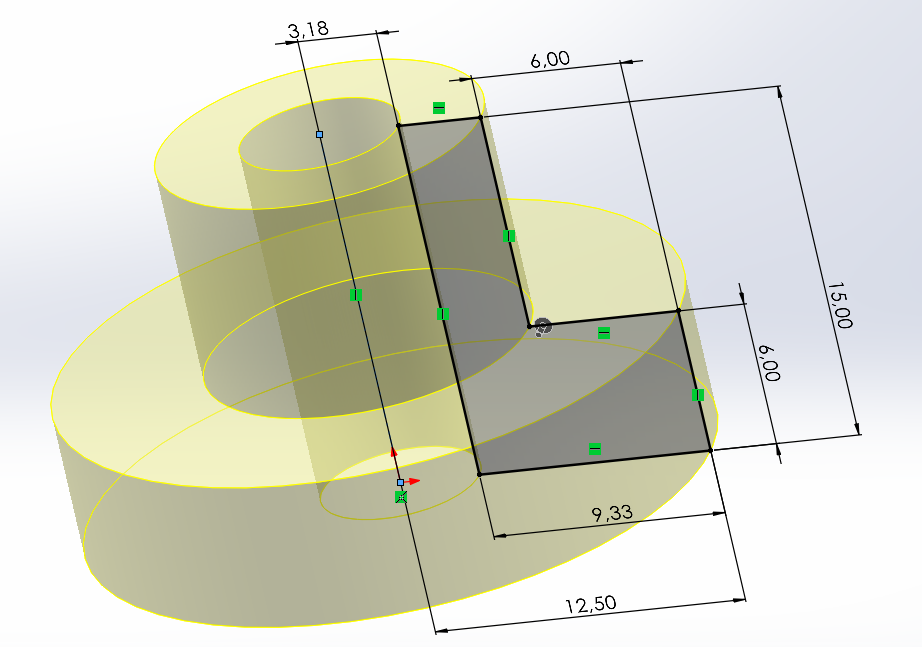
\includegraphics[width=\textwidth]{Figures/ecrou_esquisse.png}
                    \caption{Esquisse et bossage avec révolution}
                \end{subfigure}
                \hfill
                \begin{subfigure}[t]{0.4\textwidth}
                    \centering
                    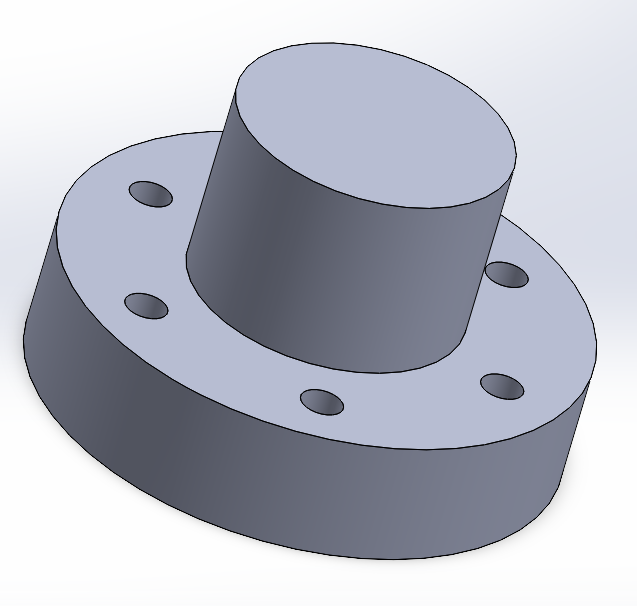
\includegraphics[width=\textwidth]{Figures/ecrou_trou.png}
                    \caption{Rajout des trous par révolution d'esquisse pour acceuillir les câbles}
                    \label{fig:vis_sans_fin_solidworks}
                \end{subfigure}
                \caption{Dessin de l'écrou}
                \label{fig:ecrou}
            \end{figure}

            Dans un premier temps, nous dessinons la forme de l'écrou hélicoïdale de la vis sans fin (voir figure \ref{fig:ecrou}), selon le modèle de la marque Igus que nous disposons. Ces écrous sont optimisés pour maximiser l'absorption des forces axiales. \cite{noauthor_bague_nodate} Le cylindre supérieure est de rayon $6.5$ mm. Enfin, nous complétons la pièce en ajoutant le filetage hélicoïdale de $6.35$ mm, égal au rayon de l'axe de la vis mère.

    \subsection{Simulation et étude de l'élasiticité via \textit{SolidWorks Simulation}}

        On crée une nouvelle étude statique. \texttt{Déplacements imposés} permet de définir les conditions limites (géométrie fixe = encastrement). \textit{Chargements externes} permet d'appliquer des forces. Enfin, il faut créer un maillage puis appuyer sur exécuter.

        Pour lancer plusieurs simulation, on utilise \texttt{étude de conception}. On rajoute une variable qu'on lie à la force et que l'on fait varier entre 1 N et 20 N, avant de créer un nouveau capteur sur le maximum de la contrainte de Von-Mises. En effet, les auteurs de \cite{bhat_numerical_2025} utilisent la contrainte équivalente linéarisée, basée sur le critère de Von-Mises. Ils ont remarqué que les contraintes sont généralement plus élevées dans la partie centrale de l'actionneur en raison des déformations plus importantes dans cette région, ce qui entraîne des contraintes plus élevées.
    
    \bibliographystyle{IEEEtran}
    \bibliography{references}

\end{document}